% !TeX program = pdflatex
% !BIB program = bibtex
\documentclass[12pt]{article}
\usepackage{epsfig}
\usepackage{subfigure} \usepackage{colortbl}
%\usepackage[linesnumbered,ruled,vlined]{algorithm2e}
\usepackage{subfigure} \usepackage{verbatim}
\usepackage{diagbox} \usepackage{color}
\usepackage{multirow} \usepackage{latexsym}
\usepackage{amsmath} \usepackage{amssymb}
\usepackage{amsthm} \usepackage{graphicx}
\usepackage{hyperref} %\usepackage[latin1]{inputenc}
\usepackage[T1]{fontenc} \usepackage[all]{xy}
\usepackage{subfigure}
\usepackage{multirow}
\usepackage{tikz}
\usetikzlibrary{calc}
%\usepackage{colortbl}
%\usepackage{subref}
%\usepackage[dvips]{color}
\usepackage{latexsym} \usepackage{amsmath}
\usepackage{amssymb} \usepackage{amsthm}
\usepackage{graphicx}
\usepackage{hyperref}
\usepackage{amssymb}
\usepackage{amsmath}
\usepackage{lineno}
\usepackage{float}
% Self-contained algorithm float and pseudocode commands. This avoids a
% dependency on the non-core algorithm/algorithmic packages at submission.
\newfloat{algorithm}{tbp}{loa}
\floatname{algorithm}{Algorithm}
\newenvironment{algorithmic}{%
  \begin{list}{}{\setlength{\leftmargin}{0pt}\setlength{\itemsep}{1pt}}\item[]%
}{\end{list}}
\newcommand{\STATE}{\par\noindent}
\newcommand{\FOR}[1]{\par\noindent\textbf{for} #1 \textbf{do}\par\begingroup\leftskip=1em}
\newcommand{\ENDFOR}{\par\endgroup\noindent\textbf{end for}}
\newcommand{\IF}[1]{\par\noindent\textbf{if} #1 \textbf{then}\par\begingroup\leftskip=1em}
\newcommand{\ELSE}{\par\endgroup\noindent\textbf{else}\par\begingroup\leftskip=1em}
\newcommand{\ENDIF}{\par\endgroup\noindent\textbf{end if}}
\usepackage{booktabs}
\usepackage{array}
\usepackage{tabularx}
\usepackage{enumitem}
%\usepackage[table,xcdraw]{xcolor}
\usepackage{multirow}
%\usepackage[french]{babel}
%\usepackage[latin1]{inputenc} \usepackage[T1]{fontenc}
\usepackage[all]{xy} \usepackage{lscape} \makeatletter
\hypersetup{hypertexnames=false}
\setlength{\emergencystretch}{2em}
\hbadness=10000
\newcommand{\bea}{\begin{eqnarray}}
\newcommand{\eea}{\end{eqnarray}}
\newcommand{\nn}{\nonumber}
\newcommand{\bee}{\begin{eqnarray*}}
\newcommand{\eee}{\end{eqnarray*}}
\newcommand{\lb}{\label}
\newcommand{\nii}{\noindent}
\newcommand{\ii}{\indent}
% Yellow revision marker used in the highlighted manuscript.
\newcommand{\revmark}[1]{\par\noindent\colorbox{yellow}{%
  \parbox{\dimexpr\linewidth-2\fboxsep}{\raggedright\strut\textbf{#1}}}%
  \par\smallskip}
\newtheorem{thm}{Theorem}[section]
\newtheorem{lem}{Lemma}[section]
\newtheorem{rem}{Remark}[section]
\begin{document}
\begin{center}
{\bf Anomaly Detection Algorithm for Enhanced Fraud
Identification in the Insurance Sector}\\
{\sc Mehrab Atighi$^{a}$, Sayed Jamal Mirkamali$^{b}$, 
 Amir T. Payandeh Najafabadi$^{a,}$\footnote{amirtpayandeh@sbu.ac.ir}}\\
a Department of Actuarial Science, Faculty of Mathematical
Sciences, Shahid Beheshti University,
Evin, 1983969411, Tehran, Iran.\\
b Department of Mathematics, Faculty of Science, Arak University,
3848177584, Arak, Iran.\\
\today
\end{center}
\revmark{HIGHLIGHTED REVISION: yellow markers identify added or replaced text.}
\begin{abstract}
\revmark{REVISED ABSTRACT --- original abstract replaced}
Insurance-fraud screening is a highly imbalanced and costly-to-verify problem: labels are scarce, fraudulent behaviour evolves, and investigators can review only a limited number of claims. We propose Sequential Anomaly Detection (SAD), a human-in-the-loop framework that converts an initially unlabeled claim stream into a progressively supervised detection process. SAD first aggregates heterogeneous unsupervised detectors to prioritize suspicious claims, obtains expert-verified labels for the selected cases, and then trains an ensemble of supervised learners that is updated after each data partition. Its multilayer variant places an entropy-based gate after the anomaly-voting stage so that expensive verification is concentrated on a smaller, higher-priority subset. Experiments on the public Carclaims automobile-insurance dataset compare three architectural variants, seven supervised learners, five anomaly-voting thresholds, and five model-voting thresholds. The reported results show that sequential updating and the multilayer gate improve the measured accuracy--review-load trade-off; the best reported configuration reaches 0.95 accuracy while reducing the number of claims forwarded for verification as thresholds become stricter. A component ablation isolates the effect of EAD inclusion and placement, while a sensitivity analysis examines the two voting thresholds and partition-wise updating. Because the available benchmark is static and single-domain, the conclusions are restricted to within-dataset validation; independent cross-dataset validation remains necessary before operational deployment.
 \end{abstract}


\noindent{\bf Keywords:} Insurance fraud detection; Sequential learning;
Human-in-the-loop learning; Anomaly detection; Ensemble voting;
Cost-sensitive screening; Multilayer architecture.

{\bf MSC2010}: {62D05, 62F10, 62N01, 65C05.}

\section{Introduction}

%   Fraud Detection:
Fraud poses a significant ethical and financial threat to the
global insurance industry. Committed by both policyholders and, at
times, insurers themselves, fraudulent activities can have severe
consequences. As high levels of fraudulent claims lead to
substantial financial losses, insurance companies must take
proactive steps to prevent fraud to avoid increasing premiums for
all customers. Even a small percentage of dishonest policyholders
can result in higher premiums across the board. In 2019, the
European Insurance and Reinsurance Federation reported an alarming
13 billion euros in industry fraud, underscoring the urgent need
for efficient and effective fraud prevention measures \cite{A61}.

The inherent stochasticity of insurance claim losses makes
identifying suspicious and fraudulent cases a complex and
time-consuming task, often demanding significant resources. In recent years, machine learning techniques have
proven to be powerful tools in detecting insurance fraud. Both
supervised and unsupervised learning approaches have demonstrated
considerable potential in enhancing the accuracy and efficiency of
fraud detection systems \cite{A61}.



%   Insurance Industry
To address the multifaceted challenges posed by fraud, this
research concentrates on enhancing fraud detection methodologies.
Our goal is to develop more efficient and accurate techniques that
reduce the number of flagged cases while maintaining a high
detection rate. By doing so, we aim to alleviate the burden on
insurance companies and their experts, enabling them to
concentrate their efforts on the most relevant and pressing cases.

In this study, we introduce a novel sequential and multilayered
anomaly detection algorithm designed to strike a balance between
accuracy and efficiency. Our approach not only contributes to
minimizing financial losses resulting from fraudulent activities
but also helps restore trust between insurance companies and their
customers. Moreover, by improving the overall fraud detection
process, businesses can potentially reduce the substantial annual
losses they currently face. Also, we seek to provide practical
solutions that can be readily implemented in the insurance
industry, ultimately benefiting both insurance providers and
policyholders. By streamlining the fraud detection process and
mitigating the adverse effects of fraudulent activities, we strive
to create a more resilient and trustworthy insurance landscape.

%   Ideas

\revmark{REVISED/ADDED --- novelty definitions, contributions, and scope}
In this article, we present a human-in-the-loop learning framework rather
than a conventional reinforcement-learning agent. The term
\emph{sequential} denotes staged learning: an unsupervised detector ensemble
prioritizes cases in the first partition, expert-verified cases initialize the
supervised models, and those models are updated after each subsequent
partition. The term \emph{multilayer} denotes a cascade, not merely a larger
ensemble: anomaly-voting produces a candidate set, an entropy-based gate
further reduces that set, and only the remaining cases are sent for expert
verification before supervised retraining.

The principal contributions are as follows:
\begin{enumerate}[label=(\roman*),leftmargin=*]
  \item a sequential weak-to-strong supervision mechanism that converts a
  largely unlabeled claim stream into progressively expanding expert-verified
  training sets;
  \item a multilayer screening architecture that separates broad anomaly
  recall from a second entropy-based verification gate, explicitly targeting
  the operational trade-off between detection performance and investigation
  workload;
  \item two interpretable voting thresholds, $T_{AD}$ and $T_{ML}$, that allow
  insurers to tune anomaly consensus and supervised-model consensus; and
  \item a component-wise comparison of Simple-A, Simple-B, and Multilayer
  variants, together with threshold and runtime analyses.
\end{enumerate}

Unlike sequence models, SAD does not model temporal dependence within a
claim. Unlike active or reinforcement learning, it does not optimize a formal
reward or query policy. Its novelty lies in the operational orchestration of
heterogeneous anomaly detectors, targeted expert verification, supervised
ensemble voting, and repeated model updating under a limited review budget.

The study should consequently be interpreted as a benchmark demonstration of
this workflow, not as evidence of immediate production readiness. The public
dataset is static, its recorded fraud label is used as a proxy for an expert
decision, and the partition order is experimental rather than chronological.
These boundaries are made explicit to distinguish the proposed workflow from
claims of temporal causality or live investigator deployment.
    %it need more text

%   Overview
The rest of this paper is organized as the following. Section
\ref{SC:LR} provides a literature review on fraud detection in the
insurance industry. We describe our proposed algorithm in Section
\ref{SC:METHOD}. In Section \ref{SC:RESULT}, we implement the
algorithm using real-world data and present evaluation metrics.
Concluding remarks and discussions are given in Section
\ref{SC:CONCLUSION}.


\section{Literature Review}\label{SC:LR}
\revmark{REVISED SECTION --- chronological survey replaced by taxonomy}

Recent reviews show that automobile-insurance fraud research is dominated by
supervised classifiers and resampling, while comparatively fewer studies
address label scarcity, verification cost, model updating, and investigation
capacity as parts of one workflow \cite{A61,Schrijver2024}. We therefore
organize the literature by learning paradigm rather than presenting a
chronological list.

\subsection{Supervised approaches}
Supervised studies learn a decision boundary from previously investigated
claims. Logistic regression, support-vector machines, random forests, boosting,
and neural networks are widely used because they support direct predictive
evaluation and can exploit heterogeneous policy and claim attributes
\cite{A41,A80}. Recent insurance-specific work has emphasized class-imbalance
handling, missing-data treatment, cost-sensitive evaluation, and model
selection \cite{BanulescuRadu2024,Khalil2024,Ding2025}. These methods are
effective when reliable labels represent the current fraud mechanism, but they
can inherit historical investigation bias and may deteriorate when fraud
patterns or claim processes change. They also assume that a sufficiently large
labelled sample exists before deployment.

\subsection{Unsupervised approaches}
Unsupervised methods rank cases by deviation from learned notions of normality.
These families include isolation forests, local outlier factors, clustering,
information-theoretic scores, and spectral ranking. Representative examples
are given by \cite{A46} and \cite{A57}. Further unsupervised fraud applications
are reported by \cite{Nian2016} and \cite{Gomes2021}. Their main advantage is
that they can screen
an initially unlabeled portfolio and potentially identify previously unseen
patterns. Their principal limitation is semantic: statistical rarity is not
equivalent to fraud. Consequently, isolated detectors can produce a review set
that is too large or poorly calibrated for investigators. Consensus voting can
reduce dependence on one detector, but a flat ensemble still applies every
expensive detector to every candidate.

\subsection{Active and reinforcement learning}
When labels are costly, sequential query selection can explicitly decide which
records should be verified. Nijhuis and van Lelyveld formulate costly outlier
verification as a reinforcement-learning problem with a defined reward and
query policy \cite{A73}. Such methods directly target the value of information,
but their performance depends on reward design, exploration assumptions, and a
stable interaction protocol. We stress that SAD is not a reinforcement-learning
algorithm: it has no state-action-reward formulation. It is instead a staged
human-in-the-loop updating procedure with deterministic voting thresholds.

\subsection{Hybrid and graph-based architectures}
Hybrid systems combine complementary signals, such as clustering followed by
classification, optimized boosting, stacking, graph-derived features, or deep
and conventional learners \cite{A27}; see also \cite{Vorobyev2024} and
\cite{Ding2025}. They can capture nonlinear and relational fraud patterns,
but frequently require richer link data, substantial tuning, or a fully
labelled development set. Moreover, a higher predictive score does not by
itself solve the operational problem of deciding how many claims investigators
can review.

\subsection{Comparative positioning and research gap}
Table~\ref{tab:positioning} identifies the distinction between SAD and the main
families of related work. The unresolved gap is an end-to-end mechanism that
(a) starts when trustworthy labels are scarce, (b) limits the number of cases
requiring verification, (c) converts verified cases into supervised training
data, and (d) updates multiple classifiers as new claim batches arrive. SAD
targets this gap through the ordered composition of anomaly consensus,
entropy-based gating, expert verification, supervised ensemble voting, and
partition-wise retraining.

\begin{table}[H]
\centering
\caption{Positioning of SAD relative to representative fraud-detection approaches.}
\label{tab:positioning}
\scriptsize
\begin{tabularx}{\textwidth}{>{\raggedright\arraybackslash}p{2.05cm}>{\raggedright\arraybackslash}p{2.45cm}>{\raggedright\arraybackslash}p{2.55cm}>{\raggedright\arraybackslash}X>{\raggedright\arraybackslash}X}
\toprule
Approach & Representative studies & Learning signal & Principal strength & Limitation addressed by SAD \\
\midrule
Supervised and cost-sensitive & Ding et al. (2025) & Historical fraud labels & Strong predictive discrimination and interpretable benchmarking & Requires an adequate labelled sample before screening and is usually trained as a static model \\
Unsupervised anomaly ranking & Nian et al. (2016) & Distributional deviation & Can discover candidates without fraud labels & Rarity is not fraud; one-stage rankings may create an impractical review workload \\
Active verification / RL & Nijhuis and van Lelyveld (2023) & Reward from selected verification & Explicitly values costly labels & Requires a formal reward and query policy; SAD instead uses transparent deterministic thresholds \\
Hybrid and graph models & Vorobyev (2024) & Labels plus relational or learned representations & Captures complex interactions and networks & Often requires linked data or extensive tuning and does not inherently constrain investigator workload \\
Proposed SAD & This study & Anomaly consensus $\rightarrow$ expert-verified labels $\rightarrow$ updated supervised ensemble & Starts with scarce labels, supports staged updating, and exposes a controllable review-performance trade-off & Needs prospective deployment and independent cross-dataset validation \\
\bottomrule
\end{tabularx}
\end{table}

\iffalse
Insurance fraud detection is a critical task for data science and
machine learning. Given the inherent complexities of the problem,
the application of various machine learning techniques for fraud
detection in the insurance industry has gained significant
attention.

Han et al. (2011) stressed the importance of clustering,
classification, and outlier analysis as crucial methods in their
work, serving as a foundational reference for understanding core
data mining challenges \cite{A71}. Ngai et al. (2011) investigated
data mining techniques in financial fraud detection, presenting a
classification framework and an extensive literature review that
compiles key methods and applications \cite{A76}.

Aggarwal et al. (2015) explored the various applications of data
mining techniques in financial fraud detection, demonstrating how
these methods can substantially improve fraud detection accuracy
\cite{A70}. Aggarwal and Philip (2015) offered a thorough review
of AI techniques in fraud detection, emphasizing the role of
machine learning methods in advancing fraud detection systems
\cite{A74}.

In a recent study, Yao et al. (2019) applied the Hampel Filter to
eliminate profile-isolated outliers in laser vision measurement,
highlighting the importance of outlier detection in enhancing
measurement accuracy \cite{A80}. Moreover, Moon et al. (2019)
employed predictive modeling for identifying fraudulent automobile
insurance claims, leveraging advanced machine learning algorithms
to enhance fraud detection effectiveness \cite{A80}. These studies
emphasize the ongoing advancements in outlier detection and
predictive modeling techniques, demonstrating their potential in
addressing fraud-related challenges in various domains, including
insurance.


Bryant and Desai (2020) further expanded on this discussion by
focusing on the practical applications of machine learning in
financial fraud detection, emphasizing the pivotal role these
technologies play in modern fraud prevention strategies
\cite{A75}. More recently, Kou et al. (2021) explored AI-based
fraud detection in the insurance and financial industries,
offering valuable insights into the integration of AI in fraud
detection systems to bolster efficiency and accuracy \cite{A78}.
These studies highlight the increasing importance of machine
learning and AI in the realm of fraud detection, showcasing their
potential to revolutionize traditional fraud prevention approaches
and enhance overall system performance.


In a recent study, Zhang et al. (2022) delved into the development
of auto insurance knowledge graphs and their application in fraud
detection, exhibiting substantial progress in leveraging knowledge
graphs for practical fraud identification purposes \cite{A27}.
Their work contributes to the ongoing advancements in data-driven
fraud detection techniques, emphasizing the importance of
integrating domain-specific knowledge for enhanced performance.


In a recent contribution, Nijhuis and van Lelyveld (2023)
investigated the application of reinforcement learning for outlier
detection in costly-to-verify data, proposing novel methods to
tackle the challenges associated with outlier handling \cite{A73}.
Their work signifies the importance of exploring advanced machine
learning techniques to overcome practical constraints and improve
the accuracy of fraud detection systems.

Collectively, these studies underscore the potential of employing
diverse machine learning and AI techniques to enhance insurance
fraud detection, augmenting the precision and efficiency of
detection systems. The research emphasizes the importance of
continued exploration and development of advanced methodologies to
address the challenges posed by insurance fraud effectively.


\fi
\section{Methodology}\label{SC:METHOD}
\revmark{REVISED/ADDED --- notation and stage ordering}
Let $D=\{(x_i,y_i)\}_{i=1}^{n}$ denote the available claim records, where
$x_i$ is the feature vector and $y_i\in\{0,1\}$ is unavailable to the
screening procedure until the claim is verified. After feature screening,
$D$ is divided into $m$ disjoint partitions $D_1,\ldots,D_m$. The first
partition initializes SAD; partitions $D_2,\ldots,D_m$ are processed in order
and the supervised ensemble is updated after each verification round. This
section defines preprocessing, the anomaly and supervised ensembles, the two
voting thresholds, and the simple and multilayer SAD architectures.

\subsection{Preprocessing}\label{SSC:PreProcessing}
Preprocessing removes uninformative predictors before partitioning the data.
The operation is feature screening rather than projection-based dimensionality
reduction: categorical variables are filtered by Gini impurity and numerical
variables by a near-zero-variance rule. Algorithm~\ref{algo:preprocessing}
summarizes the procedure.
\subsubsection*{Feature screening}

\textbf{\small Gini Index:} The Gini index measures inequality in
a dataset, ranging from 0 (all observations are equal) to 1 (all
observations are different). It's calculated by $Gini(Y) = 1 -
\displaystyle\sum_{r=1}^{R} P_r^2,$ where the lower values
indicate the more equal distribution \cite{A59}.

\textbf{Near Zero Variance:} The Near Zero Var function identifies
predictors with limited variability, such as single-value or
low-variance predictors, and those with a high frequency ratio
between the most common and second most common values \cite{A59}.
        \begin{algorithm}[H]
            \footnotesize
            \caption{PreProcessing Algorithm}\label{algo:preprocessing}
            \begin{algorithmic}
                \STATE \textbf{inputs} :  Dataset D ,   Partitioning percentages $p_i \,, i = 1, \cdots , m$ ,\\ bounds for Gini Index $g_{L} \, , g_{U}$,
                \STATE \textbf{outputs}: Partitions $D_i$, $ i = 1, \cdots , m$,
                \STATE Remove The Categorical columns of $D$ where Gini Index is not between $g_{L} \, , g_{U}$,
                \STATE Remove The Numerical columns of $D$ where Near, Zero Variance is TRUE,
                \STATE Separate  $D$ into m Partitions where the size, of $D_i$ is proportional to $p_i \,, i = 1, \cdots , m$.
            \end{algorithmic}
        \end{algorithm}

\subsubsection*{Balancing}
\revmark{REVISED --- training-only SMOTE protocol}
        \textbf{\small Resampling structures:}\\
The Synthetic Minority Over-sampling Technique (SMOTE,) is an
approach used to balance imbalanced datasets by generating
synthetic samples from the minority class. SMOTE operates by
randomly selecting a sample from the minority class and
identifying one of its k-nearest neighbors. A synthetic sample is
then generated through interpolation between these two samples.
This technique enhances the performance of machine learning models
when dealing with imbalanced data \cite{A62}.
We apply SMOTE only to each accumulated training set after the evaluation
partition has been separated. Thus, synthetic observations cannot enter the
held-out partition or leak information into its predictions.

\subsection{SAD architecture}
\revmark{REVISED/ADDED --- sequential and multilayer distinction}
We now introduce a schematic representation of two distinct
structures within our proposed Sequential Anomaly Detection (SAD)
algorithm, designed specifically for fraud identification in the
insurance industry. These structures form the basis of our
innovative approach to tackling fraudulent activities within this
domain.

Figure \ref{figai1} illustrates a sequential process
involving several stages: First, input data undergoes
preprocessing to reduce its size and is subsequently divided into
desired subsets. Anomaly detection is then applied to the first
subset, with the identified potential fraud cases sent to an
expert for verification. This step also enables fraud pattern
recognition and the development of a trained model using machine
learning algorithms. In subsequent iterations, the trained model
is employed to detect potential fraud data, allowing for expert
confirmation and continuous refinement of the machine learning
algorithms to achieve a more accurate fraud detection system.\\
Figure~\ref{figai2} illustrates the multilayer architecture. In contrast to
Simple-B, which applies EAD as one member of a flat anomaly ensemble, the
multilayer variant first constructs a consensus candidate set and only then
applies EAD as a second-stage gate. This ordered cascade is the defining
multilayer contribution because it avoids applying the more expensive gate to
every claim.

%% اینجا یک توضیح درمورد فرآیند کارو گام ها اضافه بشود.

    \begin{center}
        \begin{figure}[H]%% placement specifier
            \centering
            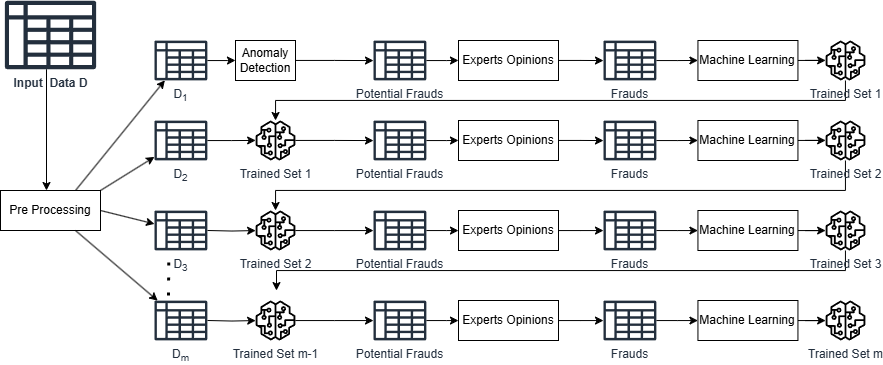
\includegraphics[width=\textwidth]{Pictures/simple.png}
    \caption{Workflow of simple structure of sequential anomaly
detection. (SAD)}\label{figai1}
           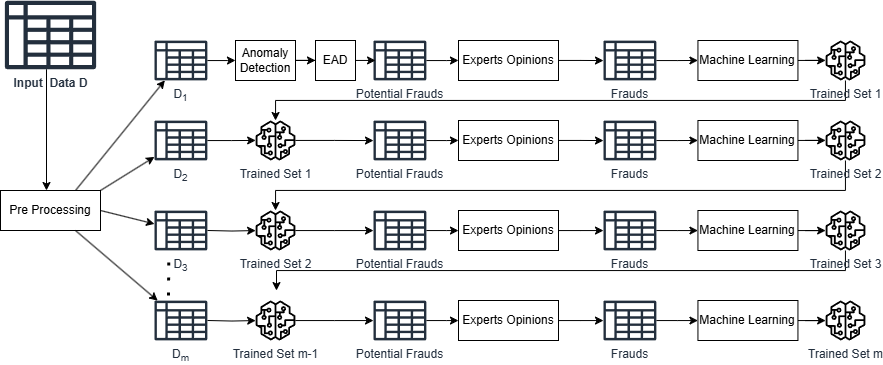
\includegraphics[width=\textwidth]{Pictures/Multilayered.png}
\caption{Workflow of multilayered structure of sequential anomaly
detection.(SAD)}\label{figai2}
        \end{figure}
    \end{center}

\subsection{Anomaly detection}\label{SSC:AD}
In the initial stage of the algorithm, the absence of reliable
labels for fraud or suspicious data necessitates unsupervised
models and techniques to identify potential fraudulent activities.
Various anomaly detection algorithms have been proposed by
researchers, and the models employed in our study are introduced
below.

\textbf{\small Box Plot:} Box plots aid in identifying outliers by
examining values that fall outside the range of $Q3 + (1.5 \times
IQR)$ or $Q1 - (1.5 \times IQR)$, where $Q1$ and $Q3$ represent
the first and third quartiles, respectively, and $IQR$ is the
interquartile range. Extreme points are defined as those beyond
$Q3 + (3 \times IQR)$ or $Q1 - (3 \times IQR)$ \cite{A4}.

\textbf{\small Percentile structure:} Percentiles partition data
into 100 segments, indicating the percentage of data points that
fall below a specific value. The $25_{th}$ percentile, for
instance, marks the point where $25\%$ of the data lies below it.
Outliers typically fall below the $5_{th}$ percentile or above the
$95_{th}$ percentile, meaning that normal data usually resides
within the $(5, 95)\%$ range \cite{A38}.

\textbf{\small Z Score structure:} Z Score identifies outliers by
comparing individual data points to the mean and standard
deviation of the dataset. Values with a Z Score above 3 or below
-3 are considered outliers. This straightforward method proves
effective when dealing with data exhibiting a normal distribution
\cite{A38}.

\textbf{\small Hample filter structure:} The Hampel Identifier
detects outliers using the median and median absolute deviation.
For data sequences with a moving window, a point is an outlier if
its difference from the local median exceeds a certain threshold.
Usually, the threshold is set to 3. If set to 0, it acts like a
standard median filter \cite{A42}.

\textbf{\small E Grubs test structure:} The Grubb's test detects
outliers in normally distributed data by contrasting the test
statistic against a critical value. It operates under the
assumption that the data contains either no outliers or a single
outlier. This test is brief and easy to implement \cite{A44}.

\textbf{\small KNN structure:} The K-Nearest Neighbors (KNN)
algorithm calculates the distance between a test instance and
training examples to identify its closest neighbors. While this
process can be computationally intensive for large datasets,
various indexing techniques can help improve its efficiency
\cite{A46}.

\textbf{\small Local outlier factor (LOF) structure:} Local
Outlier Factor (LOF) detects outliers by employing KNN to compare
each data point with its neighbors, evaluating the isolation of a
point based on its local reachability density. A simplified LOF
approach, while more computationally demanding, utilizes KNN
distance to facilitate density estimation, resulting in improved
performance \cite{A46}.

\textbf{\small Isolation forest structure:} The Isolation Forest
(iForest) algorithm efficiently detects outliers by constructing
binary trees from random dataset partitions, calculating anomaly
scores for each data point. It exhibits linear time complexity and
high precision \cite{A52}

\textbf{\small K Modes structure:} The K Modes clustering
algorithm, an alternative to K-means, efficiently clusters
categorical data by iteratively selecting k centroids, calculating
dissimilarity, assigning objects to the nearest centroid, and
updating centroids. This straightforward approach ensures optimal
clustering performance \cite{A60}.

\revmark{REVISED --- corrected Shannon entropy definition}
\textbf{\small Entropy Anomaly Detection (EAD):} Anomaly detection
using information theory calculates a dataset's information
content and observes changes when removing potential anomalies.
Higher information gain, defined as $\operatorname{Gain}(x) =
H(D)-H(D\setminus\{x\}),$ indicates an anomaly. Here, Shannon entropy is
$H(D)=-\sum_{z\in D}p(z)\log p(z)$
\cite{A57}.

Identifying anomalies can be achieved by eliminating instances
with the highest Gain(X). Efficient approximations are employed to
address the computational complexity associated with this process.

\textbf{\small Threshold limits:} In anomaly detection, it is
essential to introduce suspicious cases identified by most
methods. This is achieved using the anomaly detection threshold
limit, denoted as $T_{AD}$, which determines the criteria for
classifying data points as potential anomalies.

% باید ترش هولد را اینجا اضافه بکنیم توضیحاتش رو
%%%%%%%%%%%%%%%%%%%%%%%%%%%%%%%%%%%%%%%%%%%%%%%%%%%%%%%%%%%%%%%%%%%%%%%%%%%%%%%%%%%%%%%%%%%%%%%%%%%%%%%%%%%%%%%%%%%%%%%%%%%%%%%%%%%%%%%%%%%%%%%%%%%%%%%%%%%%%%%%%%%

\subsection{Supervised learning}\label{SSC:ML}
Following anomaly detection, the data is labeled with expert
opinions, enabling the application of supervised learning. Our
supervised learning algorithm utilizes various machine learning
techniques, which are outlined in subsequent sections.

\textbf{\small LR models:} Logistic Regression (LR) is a popular
supervised learning model used to predict outcomes based on input
features and target variables \cite{A52}.

\textbf{\small SVM models:} The Support Vector Machine (SVM) is a
widely used machine learning classifier in various real-world
applications, addressing both linear and nonlinear problems. It
separates instances of classes using a hyperplane, making it ideal
for nonlinear classification and complex problems \cite{A52}.

    \textbf{\small XGB models:}
XGBoost is an efficient gradient boosting implementation that
builds additive models using decision trees. It creates an
ensemble of base learners by iteratively minimizing errors,
outperforming individual classifiers. \cite{A57}.

    \textbf{\small RF models:}
Breiman in 2001 introduced the Random Forest (RF) classifier which
combines bagging and subspaces to construct a set of decision
trees from the training dataset. Predictions are made based on
votes from these trees, yielding high accuracy.
\cite{A52}.

\textbf{\small NB models:} Na\"ive Bayes (NB) is an efficient
predictive model for large datasets, utilizing Bayes' theorem and
assuming predictor independence. In fraud detection, the model
calculates probabilities with Maximum A Posteriori (MAP) and is
distinct due to its feature distribution assumptions \cite{A52}.

    \textbf{\small ADAB Boost models:}
Adaptive Boosting, or Adaboost, is a renowned machine learning
algorithm known for its quick boosting capabilities. Boosting
algorithms transform lazy learners into eager learners, enhancing
their predictive abilities through training\cite{A52}.

    \textbf{\small ANN models:}
Artificial Neural Networks (ANNs) are models inspired by the human
brain, capable of learning patterns from data and making
predictions. ANNs comprise interconnected artificial neurons
processing information through layers. By adjusting weights and
biases, they adapt to complex data relationships \cite{A52}.


    \textbf{\small Threshold limit:}
In machine learning methods, it is crucial to identify cases that
most algorithms have flagged as suspicious under the potential
frauds category. This is accomplished using the machine learning
threshold limit, denoted as $T_{ML}$, which establishes the
criteria for classifying data points as potential fraud cases.

\subsection{Sequential Anomaly Detection (SAD)}\label{SSC:SAD}
\revmark{REVISED/ADDED --- formal voting rules and updating sequence}
SAD is sequential because its training information grows across ordered data
partitions. It is multilayer only when the anomaly consensus and EAD gate are
applied as distinct consecutive stages. Let $a_{ik}\in\{0,1\}$ denote the vote
of anomaly detector $k$ for record $i$ and let $s_{i\ell}\in\{0,1\}$ denote
the vote of supervised model $\ell$. A first-partition record is shortlisted
when $\sum_{k=1}^{N}a_{ik}\geq T_{AD}$; in the multilayer variant, the EAD gate
must additionally accept it. For $j\geq2$, a record is shortlisted when
$\sum_{\ell=1}^{M}s_{i\ell}\geq T_{ML}$. Verified labels are accumulated before
training the next partition's ensemble. Algorithms~\ref{algo:simple} and
\ref{algo:multilayer} make this ordering explicit.
\subsubsection*{Simple structure of the SAD algorithm}
\label{sec4_2}  The anomaly detection process starts with
unlabeled data from the initial section. After voting-based
labeling, it predicts new instances using machine learning methods
(supervised learning). At the end of each section, models are
updated with expert opinions, enabling continuous improvement in
anomaly detection.

The structure takes multiple inputs, including the number of
machine learning models, anomaly detection methods, minimum votes
for machine learning models and anomaly detection methods, as well
as the set of machine learning models and anomaly detection
methods. Additionally, the dataset provided to Algorithm
\ref{algo:preprocessing} is a critical input for the structure.
These inputs contribute to a comprehensive preprocessing phase in
the anomaly detection process.

In the initial step, all data from the first section is processed
by anomaly detection methods. Each observation and method is
labeled as either normal (assigned a value of 0) or anomalous
(assigned a value of 1) based on the method's determination. Next,
for each observation in the first section, the labels received
from each method are summed, referred to as the total votes for
that observation, $U_{Total}$. If $U_{Total}$ is greater than or
equal to the threshold $T_{AD}$, the observation is flagged as
suspicious; otherwise, it is considered normal.

The set $F_1$ consists of all observations identified as
suspicious and is submitted to experts for further analysis. After
review, each observation in $F_1$ receives a new label (0 or 1),
indicating whether fraud is present, forming the set $E_1$. Since
$E_1$ is likely to have imbalanced labels, balancing methods are
applied to make it suitable for use in machine learning models. To
achieve better balance, $PN$ percent of normal data from the first
section is combined with the balanced $E_1$, creating the new
balanced set $E'_1$.

For each machine learning model, the balanced set $E'_1$ is used
for training, and then all observations in the second data section
are classified using each trained model. Every model contributes a
vote for each observation, and if the total votes exceed the
threshold $T_{ML}$, the observation is flagged as an outlier for
expert review. Data balancing and model updating are performed
iteratively for subsequent sections, ensuring that the models
remain current throughout the entire dataset analysis.

\par\medskip
\refstepcounter{algorithm}
\noindent\textbf{Algorithm \thealgorithm: Simple structure of the SAD
algorithm}\label{algo:simple}
\par\smallskip\hrule\smallskip
\begingroup\scriptsize
%   \begin{tikzpicture}[overlay, remember picture]
%       \draw [black, thick] ($(current page.south west) + (1.5,17.5 + 1.2)$) -- ($(current page.north west) + (1.5,-3.5 + 1.2)$) node[midway, above, sloped] {Descriptive layer};
%
%       \draw [black, thick] ($(current page.south west) + (1.5,15.3 + 1.2)$) -- ($(current page.north west) + (1.5,-11.1 + 1.2)$) node[midway, above, sloped] {RL};
%
%       \draw [black, thick] ($(current page.south west) + (1.5,13.7 + 1.2)$) -- ($(current page.north west) + (1.5,-12.8 + 1.2)$) node[midway, above, sloped] {ML};
%
%       \draw [black, thick] ($(current page.south west) + (1.5,5 + 1.2)$) -- ($(current page.north west) + (1.5,-14.3 + 1.2)$) node[midway, above, sloped] {Updating Layer};
%   \end{tikzpicture}


    \begin{algorithmic}
        \STATE \textbf{inputs} : Dataset D , AD SET , ML SET , Expert opinion , PN
        \STATE \textbf{outputs}  : trained models , potential frauds
        %%\STATE m $\gets$ Number of partitions of the input dataset.
        \STATE $N \gets$ number of anomaly detection methods.
        \STATE $M \gets$ number of machine learning models.
        \STATE AD SET $\gets$ ($AD_1 , \cdots , AD_{N} $)
        \STATE ML SET  $\gets$ ($ML_1 , \cdots , ML_{M} $)
        \STATE $T_{AD} \gets$ Threshold number of voting for anomaly detection methods
        \STATE $T_{ML} \gets$ Threshold number of voting for machine learning models
        \STATE PreProcessing on the input dataset $D$ which is described in Algorithm \ref{algo:preprocessing}
        %%\STATE Partition the input dataset $D$ into $D_1 , D_2 , ... , D_m$
        \STATE Store the result of anomaly detection methods of AD SET on $D_1$  into $U_{1} , \cdots , U_{N}$ (0 for normal \& 1 for anomaly).
        \FOR{Each row of $D_1$}
        \STATE Set $U_{Total} = \sum_{i = 1}^{N}{U_{i}}$
        \IF{$U_{Total} \ge T_{AD}$}
        \STATE Label the row as Potential Fraud
        \ELSE
        \STATE Label the row as Potential Normal
        \ENDIF
        \ENDFOR
        \STATE Create $F_1$ dataset as the subset of $D_1$  for which labeled as Potential Fraud.
        \STATE Send $F_1$ dataset for experts.
        \STATE Receive the opinion of experts on $F_1$ dataset as $E_1$
        \STATE Create $E^\prime_1$ as oversampling SMOTE model of $E_1 \cup G_1$  where $G_1$ is a random subset of size PN\% of $D_1$ for which labeled as Potential Normal
        \FOR{each Model of ML SET}
        \STATE Learn the Model with $E^\prime_1$ Dataset as training set.
        \ENDFOR
        \STATE Set trained models as $TS_1$
        \FOR{j from 2 to m}
        \FOR{each row of $D_j$}
        \STATE Use $TS_{j-1}$ for prediction on $D_j$ as the test partition.
        \STATE Store the response prediction of  $TS_{j-1}$ on $D_j$  into $V_{1} , \cdots , V_{M}$ (0 for normal \& 1 for anomaly).
        \STATE Set $V_{Total} = \sum_{i = 1}^{M}{V_{i}}$
        \IF{$V_{Total} \ge T_{ML}$}
        \STATE Label the row as Potential Fraud
        \ELSE
        \STATE Label the row as Potential Normal
        \ENDIF
        \ENDFOR
        \STATE Create $F_j$ dataset as the subset of $D_j$  for which labeled as Potential Fraud.
        \STATE Send $F_j$ dataset for experts.
        \STATE Receive the opinion of experts on $F_j$ dataset as $E_j$
        \STATE Create $E^\prime_j$ as oversampling SMOTE model of $E_j \cup G_j\, \cup E^\prime_{j-1} \, $  where $G_j$ is a random subset of size PN\% of $D_j$ for which labeled as Potential Normal
        \FOR{each Models of ML SET}
        \STATE Learn the Model with $E^\prime_j$ Dataset as training set.
        \ENDFOR
        \STATE Set trained models as $TS_j$
        \ENDFOR
    \end{algorithmic}
\endgroup
\smallskip\hrule\par\medskip


\subsubsection*{Multilayered structure of the SAD algorithm}
\label{sec4_3} The Multilayered structure of the SAD algorithm processes data from the
preprocessing algorithm \ref{algo:preprocessing}, identifying
anomalies in the unlabeled first section data through voting-based
labeling. It then predicts new instances in subsequent sections
using machine learning methods and updates models with expert
feedback at the end of each section.

The structure's inputs include: the number of machine learning
models, anomaly detection methods, minimum votes for machine
learning models and anomaly detection methods, the set of machine
learning models and anomaly detection methods, and the dataset
provided to the preprocessing algorithm \ref{algo:preprocessing}.

In the first step, all first-section data is processed by anomaly
detection methods. Each observation and method is labeled as
normal (0) or anomalous (1) based on the method's assessment.

In the subsequent step, the sum of labels from each method is
calculated for every observation in the first section, denoted as
$U_{Total}$. If $U_{Total}$ exceeds the threshold $T_{AD}$, the
observation is flagged as suspicious; otherwise, it is considered
normal.

The set $Y_1$ comprises all observations suspected of fraud. These
observations undergo re-examination using the entropy method
$EAD$. If $EAD$ also identifies them as suspicious, they are
included in the dataset $F_1$ for expert review. After expert
analysis, each observation receives a new label indicating
fraudulence (0 or 1), forming the set $E_1$.


The set $E_1$ likely contains imbalanced labels, necessitating
balancing for effective use in machine learning models. To achieve
better balance, $PN$ percent of normal data from the first section is
combined with $E_1$, yielding the balanced set $E'_1$. This
balanced set can then be utilized for training machine learning
models.

Each machine learning model is trained on the balanced dataset
$E'_1$ and then classifies observations in the second data section.
If the total votes for an observation surpass $T_{ML}$, it is
flagged as an outlier for expert review. Datasets are balanced and
models updated iteratively for subsequent sections, maintaining
optimal performance and up-to-date models throughout the process.


\par\medskip
\refstepcounter{algorithm}
\noindent\textbf{Algorithm \thealgorithm: Multilayered structure of the SAD
algorithm}\label{algo:multilayer}
\par\smallskip\hrule\smallskip
\begingroup\scriptsize
%   \begin{tikzpicture}[overlay, remember picture]
%       \draw [black, thick] ($(current page.south west) + (1.5,18.3 + 8/72)$) -- ($(current page.north west) + (1.5,-2.2 + 8/72)$) node[midway, above, sloped] {Descriptive layer};
%
%       \draw [black, thick] ($(current page.south west) + (1.5,15 + 8/72)$) -- ($(current page.north west) + (1.5,-10 + 8/72)$) node[midway, above, sloped] {Entropy};
%
%       \draw [black, thick] ($(current page.south west) + (1.5,13.3 + 8/72)$) -- ($(current page.north west) + (1.5,-13.2 + 8/72)$) node[midway, above, sloped] {RL};
%
%       \draw [black, thick] ($(current page.south west) + (1.5,11.7 + 8/72)$) -- ($(current page.north west) + (1.5,-14.9 + 8/72)$) node[midway, above, sloped] {ML};
%
%       \draw [black, thick] ($(current page.south west) + (1.5,3 + 8/72)$) -- ($(current page.north west) + (1.5,-16.6 + 8/72)$) node[midway, above, sloped] {Updating Layer};
%   \end{tikzpicture}

    \begin{algorithmic}
        \STATE \textbf{inputs} : Dataset D , AD SET , ML SET , Expert opinion , PN
        \STATE \textbf{outputs}  : trained models , potential frauds
        %%\STATE m $\gets$ Number of partitions of the input dataset.
        \STATE $N \gets$ number of anomaly detection methods.
        \STATE $M \gets$ number of machine learning models.
        \STATE AD SET $\gets$ ($AD_1 , \cdots , AD_{N} $)
        \STATE ML SET  $\gets$ ($ML_1 , \cdots , ML_{M} $)
        \STATE $T_{AD} \gets$ Threshold number of voting for anomaly detection methods
        \STATE $T_{ML} \gets$ Threshold number of voting for machine learning models
        \STATE PreProcessing on the input dataset $D$ which is described in Algorithm \ref{algo:preprocessing}
        %%\STATE Partition the input dataset $D$ into $D_1 , D_2 , ... , D_m$
        \STATE Store the result of anomaly detection methods of AD SET on $D_1$  into $U_{1} , \cdots , U_{N}$ (0 for normal \& 1 for anomaly).
        \FOR{Each row of $D_1$}
        \STATE Set $U_{Total} = \sum_{i = 1}^{N}{U_{i}}$
        \IF{$U_{Total} \ge T_{AD}$}
        \STATE Add this row into the set $Y_1$
        \ELSE
        \STATE Label the row as Potential Normal
        \ENDIF
        \ENDFOR
        \FOR{Each row of $Y_1$}
        \STATE Store the result of EAD method into $C_1$
        \IF{$C_{1} = 1$}
        \STATE Label the row as Potential Fraud
        \ELSE
        \STATE Label the row as Potential Normal
        \ENDIF
        \ENDFOR
        \STATE Create $F_1$ dataset as the subset of $Y_1$  for which labeled as Potential Fraud.
        \STATE Send $F_1$ dataset for experts.
        \STATE Receive the opinion of experts on $F_1$ dataset as $E_1$
        \STATE Create $E^\prime_1$ as oversampling SMOTE model of $E_1 \cup G_1$  where $G_1$ is a random subset of size PN\% of $D_1$ for which labeled as Potential Normal
        \FOR{each Model of ML SET}
        \STATE Learn the Model with $E^\prime_1$ Dataset as training set.
        \ENDFOR
        \STATE Set trained models as $TS_1$
        \FOR{j from 2 to m}
        \FOR{each row of $D_j$}
        \STATE Use $TS_{j-1}$ for prediction on $D_j$ as the test partition.
        \STATE Store the response prediction of  $TS_{j-1}$ on $D_j$  into $V_{1} , \cdots , V_{M}$ (0 for normal \& 1 for anomaly).
        \STATE Set $V_{Total} = \sum_{i = 1}^{M}{V_{i}}$
        \IF{$V_{Total} \ge T_{ML}$}
        \STATE Label the row as Potential Fraud
        \ELSE
        \STATE Label the row as Potential Normal
        \ENDIF
        \ENDFOR
        \STATE Create $F_j$ dataset as the subset of $D_j$  for which labeled as Potential Fraud.
        \STATE Send $F_j$ dataset for experts.
        \STATE Receive the opinion of experts on $F_j$ dataset as $E_j$
        \STATE Create $E^\prime_j$ as oversampling SMOTE model of $E_j \cup G_j\, \cup E^\prime_{j-1} \, $  where $G_j$ is a random subset of size PN\% of $D_j$ for which labeled as Potential Normal
        \FOR{each Models of ML SET}
        \STATE Learn the Model with $E^\prime_j$ Dataset as training set.
        \ENDFOR
        \STATE Set trained models as $TS_j$
        \ENDFOR
    \end{algorithmic}
\endgroup
\smallskip\hrule\par\medskip

\subsection{Evaluation}\label{SSC:EVAL}
\revmark{REVISED --- metric interpretation and reporting boundary}
At each stage, predictions are compared with verified labels using accuracy,
recall, and F1-score. Because fraud is rare, accuracy must be read together
with recall and F1-score rather than as a sufficient measure by itself. The
original experiment exported aggregate metric values but not complete
class-specific confusion matrices. We therefore report those values as
recorded and avoid reinterpreting them as fraud-class-only metrics.

\textbf{\small Accuracy/Weighted Recall metric:} Accuracy measures
the ratio of correctly predicted instances to the total number of
instances. It is calculated as $Acc=\frac{TP+TN}{TP+TN+FP+FN}$,
where TP and TN represent true positives and true negatives
(correct predictions), while FP and FN denote false positives and
false negatives (incorrect predictions), respectively \cite{A3}.

\textbf{\small F1-score  metric:} F1-score represents the harmonic
mean of precision and recall. It is calculated as
$F1=\frac{2\times P S\times R S}{PS+RS}$, providing a balanced
measure of both precision and recall \cite{A3}. Higher
F1-scores indicate better model performance, considering both
false positives and false negatives.

    \textbf{Recall/Sensitivity  metric:} Recall measures the ratio of correctly predicted positive
instances to the total number of positive instances. It is
calculated as $RS\ or\ Recall\ Score=\frac{TP}{TP+FN}$, where TP
and FN represent true positives and false negatives, respectively
\cite{A3}. Higher recall indicates a better
ability to identify positive instances.


\section{Real Data Application}\label{SC:RESULT}
\revmark{REVISED --- simulation protocol and claim limits}
%%%%%%%%%%%%%%%%%%%%%%%%%%%%%%%%%%%%%%%%%%%%%%%%%%%%%%%%%%%%%%%%%%%%%%%%%%%%%%%%%%%%%%%%%%%%%%%%%%%%%%%%%%%%%%%%%%%%%%%%%%%%%%%%%%%%%%%%%%%%%%
We evaluate SAD on a public automobile-insurance claims benchmark. The
experiment is a retrospective simulation of the proposed workflow: the stored
outcome label substitutes for the decision that an investigator would provide
after a shortlisted claim is reviewed. No live experts were queried. The four
random partitions simulate successive processing rounds, but they do not
constitute a chronological concept-drift experiment. All comparative claims in
this section are therefore restricted to this dataset and protocol.

\subsection*{Carclaims dataset}
The \textbf{\small Auto Insurance Claims Fraud Detection} dataset
on Kaggle, compiled by Anto Pravin John Bosco, contains records to
identify fraudulent insurance claims. It includes various features
related to automobile insurance policies and claims, allowing the
application of machine-learning techniques for anomaly detection.
The dataset comprises 15,420 observations and 31 features,
serves as a valuable resource for developing fraud detection
models in the insurance industry. Its binary target, \texttt{FraudFound},
contains 923 fraud records (5.99\%) and 14,497 non-fraud records (94.01\%)
\cite{dataset}. In the simulation, this target is hidden during screening and
revealed only when a selected claim reaches the verification step.

\subsection*{Experimental protocol and reproducibility boundaries}
\revmark{ADDED --- leakage controls and reproducibility boundaries}
The data are randomly divided into four non-overlapping partitions with sizes
50\%, 30\%, 10\%, and 10\%. Feature screening is fitted without using the
target, and SMOTE is applied only within the accumulated training data. The
first partition initializes the anomaly-to-verification stage; each later
partition is predicted using models trained on information available from
earlier rounds. Results are reported for the original implementation's three
architectures, component learners, and threshold grid. Since the submitted
source contains neither an independent second dataset nor the complete
prediction-level outputs needed to reconstruct additional baselines, we do not
manufacture an external-validation result. This limitation is analyzed in the
External Validity subsection.

    \begin{table}[H]
        \centering
        \small
        \caption{Frequency table for some of categorical variables}
        \scriptsize
        \begin{tabular}{lrrr}
            \hline
            \multicolumn{1}{c}{Feature} & \multicolumn{1}{c}{Category} & \multicolumn{1}{c}{Percent of Category} &\multicolumn{1}{c}{Frequency} \\
            \hline
            \multicolumn{1}{c}{\multirow{2}{*}{Sex}} & \multicolumn{1}{c}{Female} & \multicolumn{1}{c}{15.69}  &\multicolumn{1}{c}{2420} \\
            \multicolumn{1}{c}{} & \multicolumn{1}{c}{Male} & \multicolumn{1}{c}{84.31}  &\multicolumn{1}{c}{13000} \\
            \hline
            \multicolumn{1}{c}{\multirow{4}{*}{MaritalStatus}} & \multicolumn{1}{c}{Divorced} & \multicolumn{1}{c}{0.49}  &\multicolumn{1}{c}{76} \\
            \multicolumn{1}{c}{} & \multicolumn{1}{c}{Married} & \multicolumn{1}{c}{68.90} &\multicolumn{1}{c}{10625} \\
            \multicolumn{1}{c}{} & \multicolumn{1}{c}{Single} & \multicolumn{1}{c}{30.38}  &\multicolumn{1}{c}{4684} \\
            \multicolumn{1}{c}{} & \multicolumn{1}{c}{Widow} & \multicolumn{1}{c}{0.23}  &\multicolumn{1}{c}{35} \\
            \hline
            \multicolumn{1}{c}{\multirow{3}{*}{VehicleCategory}} & \multicolumn{1}{c}{Sedan} & \multicolumn{1}{c}{62.72} &\multicolumn{1}{c}{9671} \\
            \multicolumn{1}{c}{} & \multicolumn{1}{c}{Sport} & \multicolumn{1}{c}{34.75}  &\multicolumn{1}{c}{5358} \\
            \multicolumn{1}{c}{} & \multicolumn{1}{c}{Utility} & \multicolumn{1}{c}{2.54} &\multicolumn{1}{c}{391} \\
            \hline
            \multicolumn{1}{c}{\multirow{4}{*}{DriverRating}} & \multicolumn{1}{c}{1} & \multicolumn{1}{c}{25.58}  &\multicolumn{1}{c}{3944} \\
            \multicolumn{1}{c}{} & \multicolumn{1}{c}{2} & \multicolumn{1}{c}{24.65}  &\multicolumn{1}{c}{3801} \\
            \multicolumn{1}{c}{} & \multicolumn{1}{c}{3} & \multicolumn{1}{c}{25.19}  &\multicolumn{1}{c}{3884} \\
            \multicolumn{1}{c}{} & \multicolumn{1}{c}{4} & \multicolumn{1}{c}{24.58}  &\multicolumn{1}{c}{3791} \\
            \hline
            \multicolumn{1}{c}{\multirow{2}{*}{FraudFound}} & \multicolumn{1}{c}{No} & \multicolumn{1}{c}{94.01}  &\multicolumn{1}{c}{14497} \\
            \multicolumn{1}{c}{} & \multicolumn{1}{c}{Yes} & \multicolumn{1}{c}{5.99}  &\multicolumn{1}{c}{923} \\
            \hline
        \end{tabular}
    \end{table}

    \subsection*{Algorithm Specifications}
In this research, by implementing the structures and models as
mentioned below, we reached the following results.
    \begin{enumerate}
        \item Preprocessing Algorithm:\\
For all scenarios executed in this algorithm, the following values
have been considered: $$m = 4 , p_1 = 50\% , p_2 = 30\% , p_3 =
10\% , p_4 = 10\% $$

        \item Simple Structure A:\\
This is the  Simple structure of the SAD algorithm where the set of machine learning
models and outlier detection methods are as follows:
        $PN = 10\%$,
        \\ AD SET $\gets$ (Box plot, Percentile, Z-Score, Hample filter, E-Grubs test, LOF, KNN, Isolation forest, KModes),\\ ML SET $\gets$ (LR, SVM, XGBoost, KNN, RF, Adaboost, NN).

        \item Simple Structure B: \\
This is the Simple structure of the SAD algorithm where the set of machine learning
models and outlier detection methods are as follows: $PN =
10\%$,\\ AD SET $\gets$ (Box plot, Percentile, Z-Score, Hample
filter, E-Grubs test, LOF, KNN, Isolation forest, KModes, EAD),\\
ML SET $\gets$ (LR, SVM, XGBoost, KNN, RF, Adaboost, NN).

        \item Multilayered structure of the SAD algorithm:\\ The set of machine learning models and outlier detection methods for this structure are as follows:\\
        $PN = 10\%$,\\ AD SET $\gets$ (Box plot, Percentile, Z-Score, Hample filter, E-Grubs test, LOF, KNN, Isolation forest, KModes, EAD),\\ ML SET $\gets$ (LR, SVM, XGBoost, KNN, RF, Adaboost, NN).
    \end{enumerate}
    \subsection*{Predictive results}
    \revmark{REVISED --- cautious interpretation of reported metrics}
    \begin{table}[H]
        \centering
        \caption{Evaluation metrics of different algorithms along with the proposed algorithm by different partitions and structures}
        \label{table2}
        \scriptsize
        \resizebox{\textwidth}{!}{%
        \begin{tabular}{lrrrrrrrrrr}
            \hline
            &  & \multicolumn{3}{c}{Simple A} & \multicolumn{3}{c}{Simple B} & \multicolumn{3}{c}{Multilayer} \\
            \hline
            \multicolumn{1}{c}{ML Model} & \multicolumn{1}{c}{Partition} & Accuracy & F1 & \multicolumn{1}{c}{Recall}  & Accuracy & F1 & \multicolumn{1}{c}{Recall} & Accuracy & F1 & \multicolumn{1}{c}{Recall} \\
            \hline
            \multicolumn{1}{c}{\multirow{3}{*}{Adaboost}} & \multicolumn{1}{c}{2} & 0.72 & 0.83 & \multicolumn{1}{c}{0.75}  & 0.74 & 0.85 & \multicolumn{1}{c}{0.77} & 0.82 & 0.90 & \multicolumn{1}{c}{0.86} \\
            \multicolumn{1}{c}{} & \multicolumn{1}{c}{3} & 0.69 & 0.81 & \multicolumn{1}{c}{0.72} & 0.72 & 0.83 & \multicolumn{1}{c}{0.75} & 0.81 & 0.89 & \multicolumn{1}{c}{0.84} \\
            \multicolumn{1}{c}{} & \multicolumn{1}{c}{4} & 0.72 & 0.83 & \multicolumn{1}{c}{0.75}  & 0.71 & 0.83 & \multicolumn{1}{c}{0.74}  & 0.84 & 0.91 & \multicolumn{1}{c}{0.88}  \\
            \hline
            \multicolumn{1}{c}{\multirow{3}{*}{KNN}} & \multicolumn{1}{c}{2} & 0.71 & 0.82 & \multicolumn{1}{c}{0.73}  & 0.69 & 0.81 & \multicolumn{1}{c}{0.72}  & 0.73 & 0.84 & \multicolumn{1}{c}{0.75}  \\
            \multicolumn{1}{c}{} & \multicolumn{1}{c}{3} & 0.68 & 0.81 & \multicolumn{1}{c}{0.71} & 0.69 & 0.82 & \multicolumn{1}{c}{0.72}  & 0.77 & 0.86 & \multicolumn{1}{c}{0.80} \\
            \multicolumn{1}{c}{} & \multicolumn{1}{c}{4} & 0.72 & 0.84 & \multicolumn{1}{c}{0.75}  & 0.75 & 0.85 & \multicolumn{1}{c}{0.78} & 0.82 & 0.90 & \multicolumn{1}{c}{0.86} \\
            \hline
            \multicolumn{1}{c}{\multirow{3}{*}{LR}} & \multicolumn{1}{c}{2} & 0.80 & 0.89 & \multicolumn{1}{c}{0.84} & 0.77 & 0.87 & \multicolumn{1}{c}{0.81} & 0.84 & 0.91 & \multicolumn{1}{c}{0.88} \\
            \multicolumn{1}{c}{} & \multicolumn{1}{c}{3} & 0.76 & 0.86 & \multicolumn{1}{c}{0.80} & 0.80 & 0.89 & \multicolumn{1}{c}{0.84}& 0.80 & 0.88 & \multicolumn{1}{c}{0.83}  \\
            \multicolumn{1}{c}{} & \multicolumn{1}{c}{4} & 0.78 & 0.87 & \multicolumn{1}{c}{0.81} & 0.80 & 0.89 & \multicolumn{1}{c}{0.83} & 0.81 & 0.89 & \multicolumn{1}{c}{0.84}  \\
            \hline
            \multicolumn{1}{c}{\multirow{3}{*}{NB}} & \multicolumn{1}{c}{2} & 0.83 & 0.90 & \multicolumn{1}{c}{0.87} & 0.83 & 0.91 & \multicolumn{1}{c}{0.88}& 0.85 & 0.92 & \multicolumn{1}{c}{0.89}  \\
            \multicolumn{1}{c}{} & \multicolumn{1}{c}{3} & 0.81 & 0.90 & \multicolumn{1}{c}{0.85} & 0.81 & 0.90 & \multicolumn{1}{c}{0.85} & 0.85 & 0.92 & \multicolumn{1}{c}{0.88}  \\
            \multicolumn{1}{c}{} & \multicolumn{1}{c}{4} & 0.84 & 0.91 & \multicolumn{1}{c}{0.88} & 0.83 & 0.91 & \multicolumn{1}{c}{0.87} & 0.85 & 0.92 & \multicolumn{1}{c}{0.88} \\
            \hline
            \multicolumn{1}{c}{\multirow{3}{*}{ANN}} & \multicolumn{1}{c}{2} & 0.81 & 0.89 & \multicolumn{1}{c}{0.85} & 0.78 & 0.87 & \multicolumn{1}{c}{0.81} & 0.83 & 0.91 & \multicolumn{1}{c}{0.87}  \\
            \multicolumn{1}{c}{} & \multicolumn{1}{c}{3} &  0.78 & 0.88 & \multicolumn{1}{c}{0.82} & 0.81 & 0.89 & \multicolumn{1}{c}{0.85} & 0.87 & 0.93 & \multicolumn{1}{c}{0.91}  \\
            \multicolumn{1}{c}{} & \multicolumn{1}{c}{4} & 0.79 & 0.88 & \multicolumn{1}{c}{0.82} & 0.80 & 0.89 & \multicolumn{1}{c}{0.84} & 0.85 & 0.92 & \multicolumn{1}{c}{0.89}  \\
            \hline
            \multicolumn{1}{c}{\multirow{3}{*}{RF}} & \multicolumn{1}{c}{2} & 0.87 & 0.93 & \multicolumn{1}{c}{0.92} & 0.86 & 0.93 & \multicolumn{1}{c}{0.92} & 0.93 & 0.96 & \multicolumn{1}{c}{0.99}  \\
            \multicolumn{1}{c}{} & \multicolumn{1}{c}{3} & 0.89 & 0.94 & \multicolumn{1}{c}{0.94} & 0.89 & 0.94 & \multicolumn{1}{c}{0.94} & 0.94 & 0.97 & \multicolumn{1}{c}{0.99} \\
            \multicolumn{1}{c}{} & \multicolumn{1}{c}{4} & \textbf{0.91} & 0.95 & \multicolumn{1}{c}{0.96} & \textbf{0.92} & 0.96 & \multicolumn{1}{c}{0.97} & \textbf{0.95} & 0.97 & \multicolumn{1}{c}{1.00} \\
            \hline
            \multicolumn{1}{c}{\multirow{3}{*}{SVM}} & \multicolumn{1}{c}{2} & 0.80 & 0.89 & \multicolumn{1}{c}{0.84} & 0.78 & 0.87 & \multicolumn{1}{c}{0.82} & 0.78 & 0.88 & \multicolumn{1}{c}{0.85}  \\
            \multicolumn{1}{c}{} & \multicolumn{1}{c}{3} & 0.74 & 0.85 & \multicolumn{1}{c}{0.78} & 0.79 & 0.88 & \multicolumn{1}{c}{0.83} & 0.72 & 0.84 & \multicolumn{1}{c}{0.75}  \\
            \multicolumn{1}{c}{} & \multicolumn{1}{c}{4} & 0.78 & 0.87 & \multicolumn{1}{c}{0.81} & 0.80 & 0.89 & \multicolumn{1}{c}{0.83} & 0.77 & 0.87 & \multicolumn{1}{c}{0.80}   \\
            \hline
            \multicolumn{1}{c}{\multirow{3}{*}{XGBoost}} & \multicolumn{1}{c}{2} & 0.82 & 0.90 & \multicolumn{1}{c}{0.87} & 0.79 & 0.88 & \multicolumn{1}{c}{0.83} & 0.71 & 0.83 & \multicolumn{1}{c}{0.74}  \\
            \multicolumn{1}{c}{} & \multicolumn{1}{c}{3} & 0.84 & 0.91 & \multicolumn{1}{c}{0.88} & 0.85 & 0.92 & \multicolumn{1}{c}{0.90} & 0.78 & 0.87 & \multicolumn{1}{c}{0.80}  \\
            \multicolumn{1}{c}{} & \multicolumn{1}{c}{4} & 0.83 & 0.91 & \multicolumn{1}{c}{0.87} & 0.86 & 0.92 & \multicolumn{1}{c}{0.91} & 0.71 & 0.83 & \multicolumn{1}{c}{0.74}  \\
            \hline
            \multicolumn{1}{c}{\multirow{3}{*}{SAD}} & \multicolumn{1}{c}{2} & \textbf{0.88} & 0.94 & \multicolumn{1}{c}{0.93} & \textbf{0.89} & 0.94 & \multicolumn{1}{c}{0.95} & \textbf{0.93} & 0.96 & \multicolumn{1}{c}{0.99}  \\
            \multicolumn{1}{c}{} & \multicolumn{1}{c}{3} & \textbf{0.89} & 0.94 & \multicolumn{1}{c}{0.94} & \textbf{0.91} & 0.95 & \multicolumn{1}{c}{0.96} & \textbf{0.94} & 0.97 & \multicolumn{1}{c}{0.99}  \\
            \multicolumn{1}{c}{} & \multicolumn{1}{c}{4} & \textbf{0.94} & \textbf{0.97} & \multicolumn{1}{c}{0.99} & \textbf{0.94} & \textbf{0.97} & \multicolumn{1}{c}{\textbf{0.99}} & \textbf{0.95} & \textbf{0.97} & \multicolumn{1}{c}{\textbf{1.00}}  \\
            \hline
        \end{tabular}}
    \end{table}
Table~\ref{table2} compares the component learners with the ensemble output
reported as SAD. Random forest is the strongest individual learner in most
settings, while the SAD vote provides the highest or joint-highest reported
accuracy across the three architectures. In partition 4, SAD reaches reported
accuracy values of 0.94, 0.94, and 0.95 for Simple-A, Simple-B, and Multilayer,
respectively. The multilayer configuration also attains the largest reported
F1-score (0.97) and recall (1.00) in that partition. These values describe this
particular random-partition run; without repeated-run uncertainty intervals or
fraud-class confusion matrices, small differences should not be interpreted as
proof of universal superiority.

\subsection*{Component ablation and threshold sensitivity}
\revmark{ADDED --- formal component ablation and sensitivity analysis}
The three structures form a component ablation. Simple-A omits EAD, Simple-B
adds EAD as a tenth member of the flat anomaly ensemble, and Multilayer moves
EAD into a second-stage gate after the nine-detector consensus. Holding the
supervised learner set, partitions, and normal-sampling percentage fixed
isolates the architectural role of the EAD component and its placement.
    \begin{table}[H]
        \centering
        \caption{Component ablation and threshold sensitivity of SAD across the three architectures}
        \label{table3}
        \scriptsize
        \begin{tabular}{rrrrrrrrrrr}
            \hline
            &&\multicolumn{3}{c}{Simple A} &  \multicolumn{3}{c}{Simple B} &  \multicolumn{3}{c}{MultiLayer} \\
            \hline
            \multicolumn{1}{c}{$T_{ML}$} & \multicolumn{1}{c}{$T_{AD}$} & F1 & Recall & \multicolumn{1}{c}{Accuracy}  & F1 & Recall & \multicolumn{1}{c}{Accuracy}  & F1 & Recall & \multicolumn{1}{c}{Accuracy}\\
            \hline
            \multicolumn{1}{c}{\multirow{5}{*}{3}} & \multicolumn{1}{c}{1}& 0.54 & 0.38 & \multicolumn{1}{c}{\textbf{0.39}} & 0.54 & 0.38 & \multicolumn{1}{c}{0.39}  & 0.78 & 0.67 & \multicolumn{1}{c}{0.65} \\
            \multicolumn{1}{c}{} & \multicolumn{1}{c}{2}& 0.57 & 0.41 & \multicolumn{1}{c}{\textbf{0.42}} & 0.60 & 0.44 & \multicolumn{1}{c}{0.45} & 0.79 & 0.67 & \multicolumn{1}{c}{0.65} \\
            \multicolumn{1}{c}{} & \multicolumn{1}{c}{3}& 0.77 & 0.64 & \multicolumn{1}{c}{\textbf{0.63}} & 0.77 & 0.54 & \multicolumn{1}{c}{0.54} & 0.79 & 0.67 & \multicolumn{1}{c}{0.66}\\
            \multicolumn{1}{c}{} & \multicolumn{1}{c}{4}& 0.84 & 0.75 & \multicolumn{1}{c}{\textbf{0.72}} & 0.69 & 0.78 & \multicolumn{1}{c}{0.75} & 0.84 & 0.76 & \multicolumn{1}{c}{0.73} \\
            \multicolumn{1}{c}{} & \multicolumn{1}{c}{5}& 0.88 & 0.82 & \multicolumn{1}{c}{\textbf{0.79}} & 0.85 & 0.79 & \multicolumn{1}{c}{\textbf{0.76}} & 0.84 & 0.76 & \multicolumn{1}{c}{\textbf{0.73}} \\
            \hline
            \multicolumn{1}{c}{\multirow{5}{*}{4}} & \multicolumn{1}{c}{1}& 0.72 & 0.58 & \multicolumn{1}{c}{0.57}& 0.68 & 0.54 & \multicolumn{1}{c}{0.53}& 0.87 & 0.81 & \multicolumn{1}{c}{0.78} \\
            \multicolumn{1}{c}{} & \multicolumn{1}{c}{2}& 0.75 & 0.62 & \multicolumn{1}{c}{0.61} & 0.72 & 0.58 & \multicolumn{1}{c}{0.57} & 0.87 & 0.80 & \multicolumn{1}{c}{0.77}   \\
            \multicolumn{1}{c}{} & \multicolumn{1}{c}{3}& 0.88 & 0.82 & \multicolumn{1}{c}{0.79} & 0.80 & 0.69 & \multicolumn{1}{c}{0.67} & 0.92 & 0.89 & \multicolumn{1}{c}{0.85}   \\
            \multicolumn{1}{c}{} & \multicolumn{1}{c}{4}& 0.91 & 0.87 & \multicolumn{1}{c}{0.83} & 0.90 & 0.86 & \multicolumn{1}{c}{0.82} & 0.92 & 0.89 & \multicolumn{1}{c}{0.84}   \\
            \multicolumn{1}{c}{} & \multicolumn{1}{c}{5}& 0.92 & 0.90 & \multicolumn{1}{c}{\textbf{0.86}} & 0.92 & 0.89 & \multicolumn{1}{c}{\textbf{0.85}} & 0.92 & 0.90 & \multicolumn{1}{c}{\textbf{0.85}} \\
            \hline
            \multicolumn{1}{c}{\multirow{5}{*}{5}} & \multicolumn{1}{c}{1}& 0.82 & 0.73 & \multicolumn{1}{c}{0.70} & 0.80 & 0.69 & \multicolumn{1}{c}{0.67} & 0.93 & 0.91 & \multicolumn{1}{c}{0.87} \\
            \multicolumn{1}{c}{} & \multicolumn{1}{c}{2}& 0.81 & 0.71 & \multicolumn{1}{c}{0.68} & 0.82 & 0.73 & \multicolumn{1}{c}{0.70} & 0.94 & 0.92 & \multicolumn{1}{c}{0.88} \\
            \multicolumn{1}{c}{} & \multicolumn{1}{c}{3}& 0.91 & 0.88 & \multicolumn{1}{c}{0.83} & 0.88 & 0.82 & \multicolumn{1}{c}{0.79} & 0.95 & 0.96 & \multicolumn{1}{c}{0.91} \\
            \multicolumn{1}{c}{} & \multicolumn{1}{c}{4}& 0.94 & 0.93 & \multicolumn{1}{c}{0.88} & 0.93 & 0.92 & \multicolumn{1}{c}{0.88} & 0.95 & 0.95 & \multicolumn{1}{c}{0.90}  \\
            \multicolumn{1}{c}{} & \multicolumn{1}{c}{5}& 0.94 & 0.94 & \multicolumn{1}{c}{\textbf{0.89}} & 0.94 & 0.94 & \multicolumn{1}{c}{\textbf{0.89}} & 0.96 & 0.98 & \multicolumn{1}{c}{\textbf{0.93}}  \\
            \hline
            \multicolumn{1}{c}{\multirow{5}{*}{6}} & \multicolumn{1}{c}{1}& 0.88 & 0.82 & \multicolumn{1}{c}{0.78} & 0.87 & 0.81 & \multicolumn{1}{c}{0.78} & 0.96 & 0.97 & \multicolumn{1}{c}{0.92}  \\
            \multicolumn{1}{c}{} & \multicolumn{1}{c}{2}& 0.87 & 0.80 & \multicolumn{1}{c}{0.77} & 0.88 & 0.82 & \multicolumn{1}{c}{0.78} & 0.96 & 0.97 & \multicolumn{1}{c}{0.92}  \\
            \multicolumn{1}{c}{} & \multicolumn{1}{c}{3}& 0.94 & 0.94 & \multicolumn{1}{c}{0.90} & 0.93 & 0.92 & \multicolumn{1}{c}{0.87}  & 0.97 & 0.99 & \multicolumn{1}{c}{0.94} \\
            \multicolumn{1}{c}{} & \multicolumn{1}{c}{4}& 0.95 & 0.96 & \multicolumn{1}{c}{0.91} & 0.95 & 0.96 & \multicolumn{1}{c}{0.91} & 0.97 & 1.00 & \multicolumn{1}{c}{0.94}   \\
            \multicolumn{1}{c}{} & \multicolumn{1}{c}{5}& 0.96 & 0.98 & \multicolumn{1}{c}{\textbf{0.92}} & 0.96 & 0.97 & \multicolumn{1}{c}{\textbf{0.92}} & 0.97 & 1.00 & \multicolumn{1}{c}{\textbf{0.95}}  \\
            \hline
            \multicolumn{1}{c}{\multirow{5}{*}{7}} & \multicolumn{1}{c}{1}& 0.94 & 0.95 & \multicolumn{1}{c}{0.90} & 0.94 & 0.92 & \multicolumn{1}{c}{0.88} & 0.97 & 0.99 & \multicolumn{1}{c}{0.94}  \\
            \multicolumn{1}{c}{} & \multicolumn{1}{c}{2}& 0.94 & 0.93 & \multicolumn{1}{c}{0.88} & 0.93 & 0.91 & \multicolumn{1}{c}{0.87} & 0.97 & 1.00 & \multicolumn{1}{c}{0.94}  \\
            \multicolumn{1}{c}{} & \multicolumn{1}{c}{3}& 0.96 & 0.97 & \multicolumn{1}{c}{0.92} & 0.96 & 0.96 & \multicolumn{1}{c}{0.92} & 0.97 & 1.00 & \multicolumn{1}{c}{0.94}  \\
            \multicolumn{1}{c}{} & \multicolumn{1}{c}{4}& 0.97 & 0.99 & \multicolumn{1}{c}{0.94} & 0.97 & 0.97 & \multicolumn{1}{c}{0.94} & 0.97 & 1.00 & \multicolumn{1}{c}{0.95}   \\
            \multicolumn{1}{c}{} & \multicolumn{1}{c}{5}& 0.97 & 0.99 & \multicolumn{1}{c}{\textbf{0.94}} & 0.97 & 0.97 & \multicolumn{1}{c}{\textbf{0.94}} & 0.97 & 1.00 & \multicolumn{1}{c}{\textbf{0.94}} \\
            \hline
        \end{tabular}
    \end{table}
Table~\ref{table3} shows three findings. First, at the operational setting
$T_{ML}=6$ and $T_{AD}=5$, the multilayer architecture reports 0.95 accuracy,
compared with 0.92 for both flat alternatives. Second, moving EAD from the flat
ensemble (Simple-B) to the second-stage gate produces the clearest gains at
lower and intermediate threshold settings; for example, at
$(T_{ML},T_{AD})=(4,3)$, reported accuracy increases from 0.67 to 0.85. Third,
larger vote thresholds generally raise the tabulated metrics, although the
pattern is not strictly monotone in every cell. Thresholds also change the
number and composition of claims sent for verification, so the table should be
read as a sensitivity analysis of a review-performance trade-off, not as a
causal guarantee that stricter thresholds always improve fraud detection.
    %%FIG1
    \begin{center}
        \begin{figure}[H]%% placement specifier
            % Use \includegraphics command to insert graphic files. Place graphics files in
            %% working directory.
            \centering%% For centre alignment of image.
            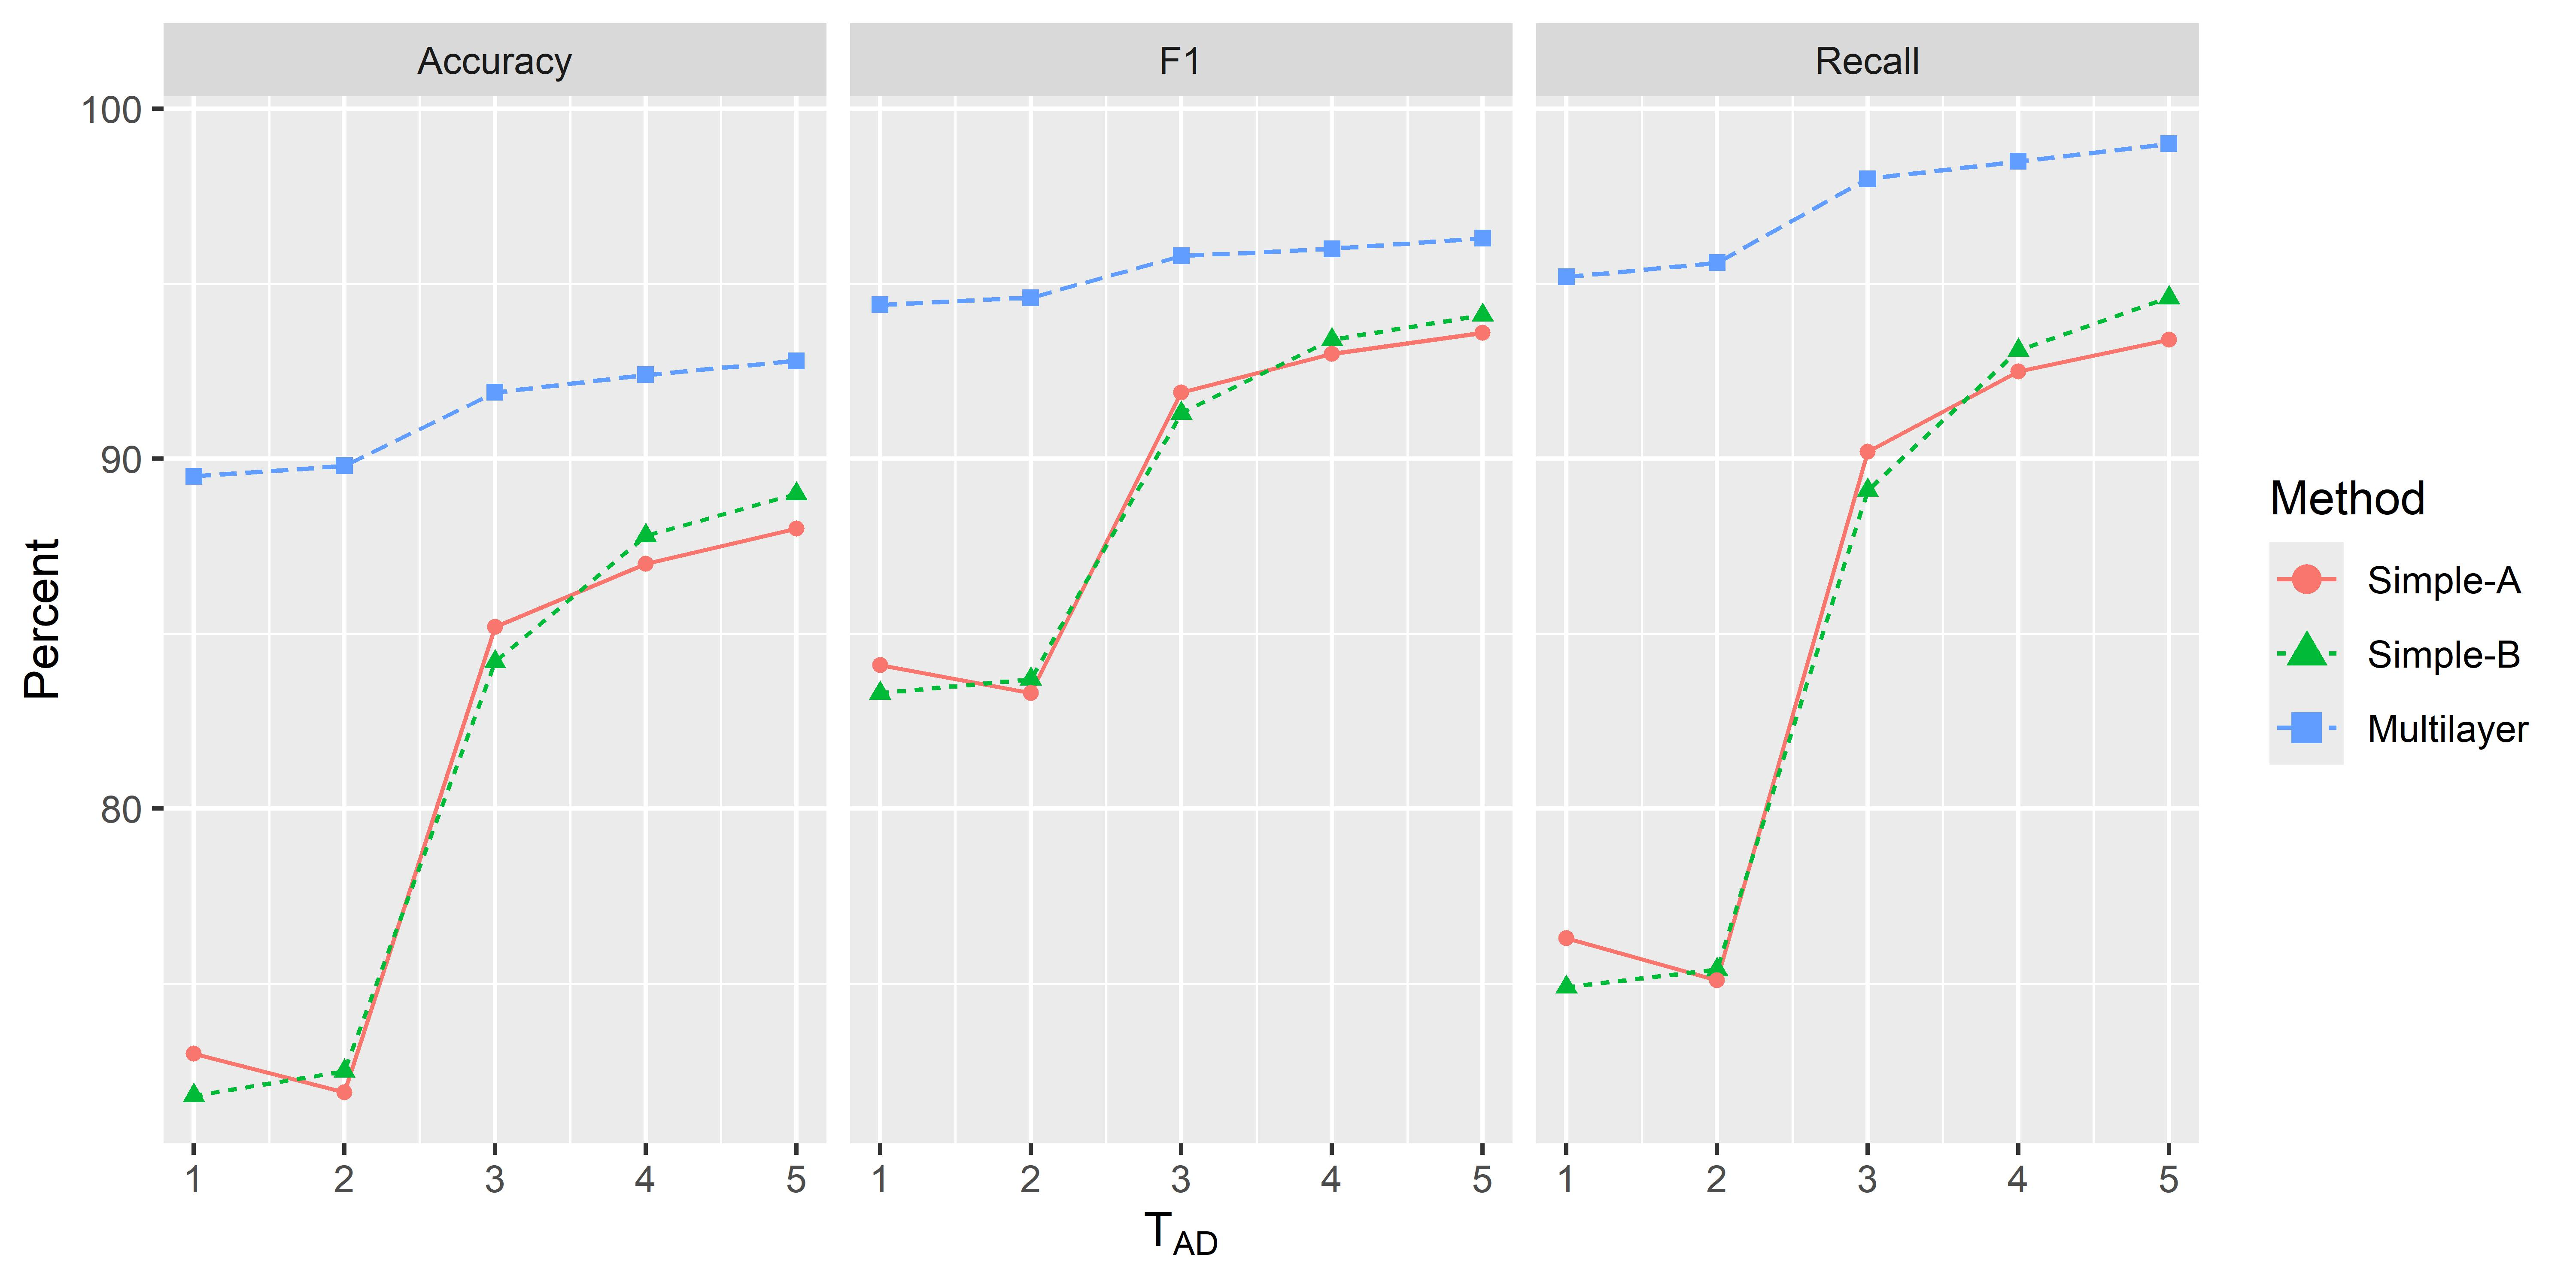
\includegraphics[width=\textwidth]{Pictures/FIG1.JPEG}
            %% Use \caption command for figure caption and label.
            \caption{The trend of evaluation metric of $SAD$ algorithm respect to $T_{AD}$ in the second partition for $T_{ML} = 7 \,, M = 8 $ and different structures}\label{fig1}
            %https://en.wikibooks.org/wiki/LaTeX/Importing_Graphics#Importing_external_graphics
        \end{figure}
    \end{center}
In Figure \ref{fig1}, with $T_{ML}$ fixed at 7 for the second
partition, it becomes evident that accuracy exhibits a positive
correlation with $T_{AD}$. Specifically, in Simple-A and Simple-B
structures, an increase in $T_{AD}$ from 2 to 3 yields a
significant upward jump in accuracy. However, the Multilayered structure of the SAD algorithm generally outperforms the other two structures. This
trend of the multilayer structure's superior performance can also
be observed in the F1-score and Recall metrics.


    %%FIG2

    \begin{center}
        \begin{figure}[H]%% placement specifier

            \centering
            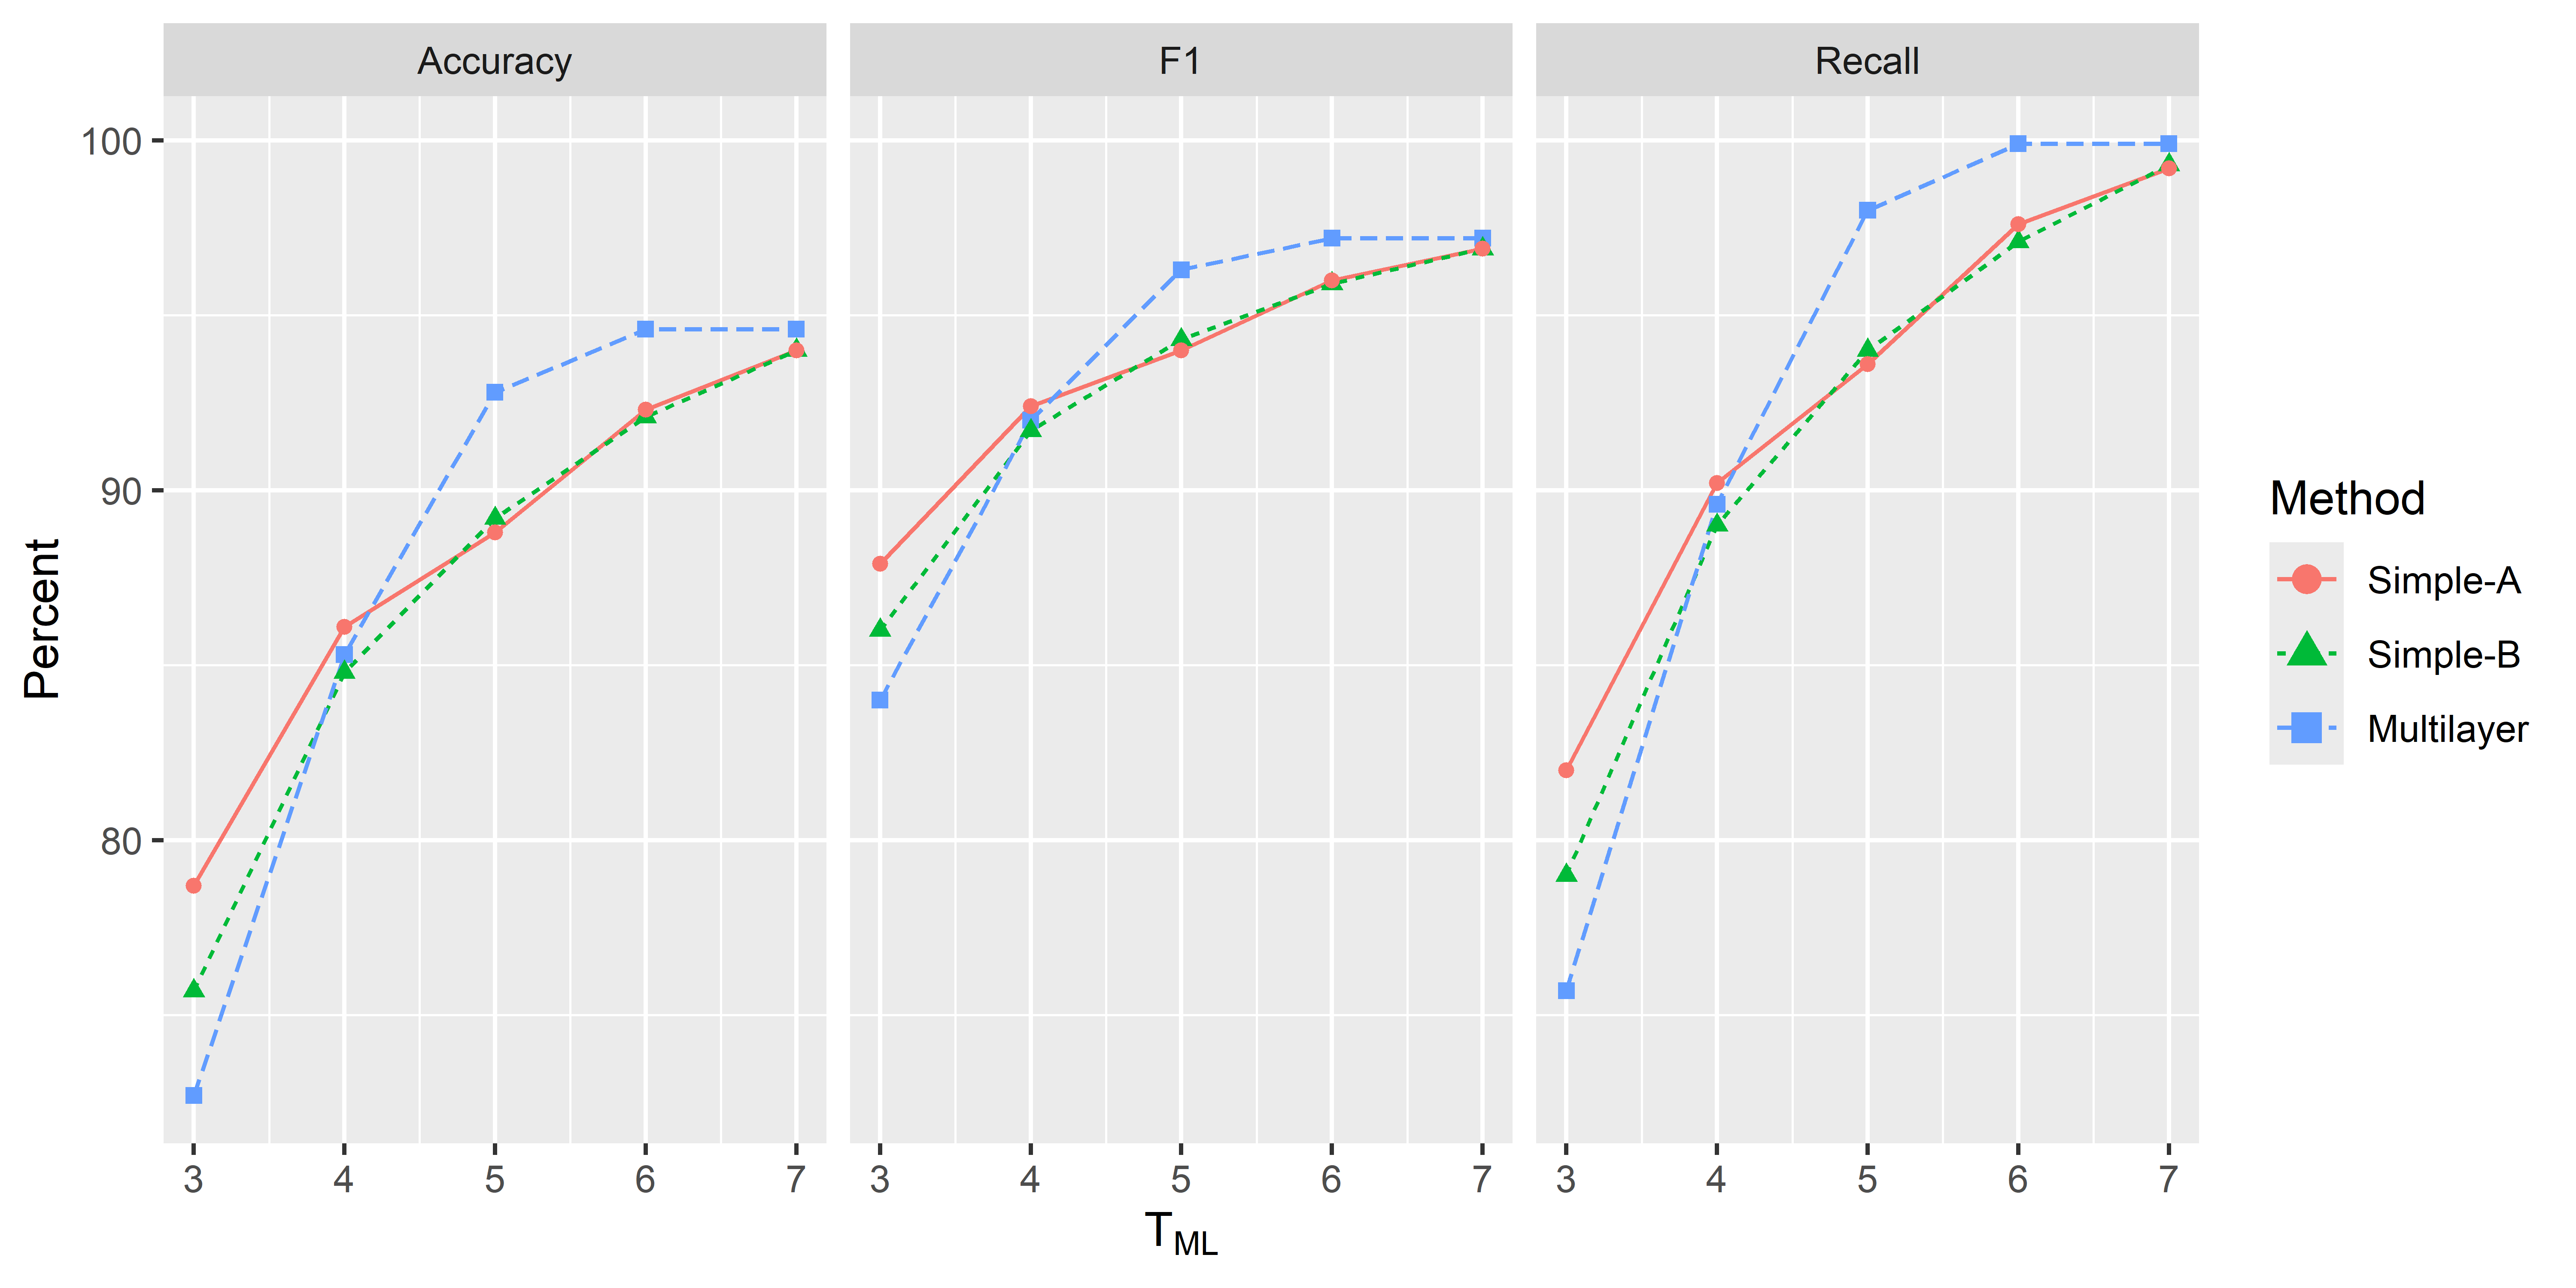
\includegraphics[width=\textwidth]{Pictures/FIG2.PNG}

            \caption{Evaluation metrics of SAD versus $T_{ML}$ in the fourth partition for $T_{AD}=5$, $M=8$, and the three architectures.}\label{fig2}

        \end{figure}
    \end{center}

In Figure \ref{fig2}, with $T_{AD}$ set to 5 for the fourth
partition, we observe that accuracy demonstrates a positive
correlation with $T_{ML}$. In Simple-A and Simple-B structures, an
increase in $T_{ML}$ from 3 to 5 results in a noticeable upward
jump in accuracy. However, the Multilayered structure of the SAD algorithm consistently
outperforms the other two structures. Similar trends can be
observed for the F1-score and Recall metrics. Notably, in the
multilayer structure, the rate of change appears to stabilize when
$T_{ML}$ reaches 6 or higher.



    %%FIG3

    \begin{center}
        \begin{figure}[H]%% placement specifier

            \centering
            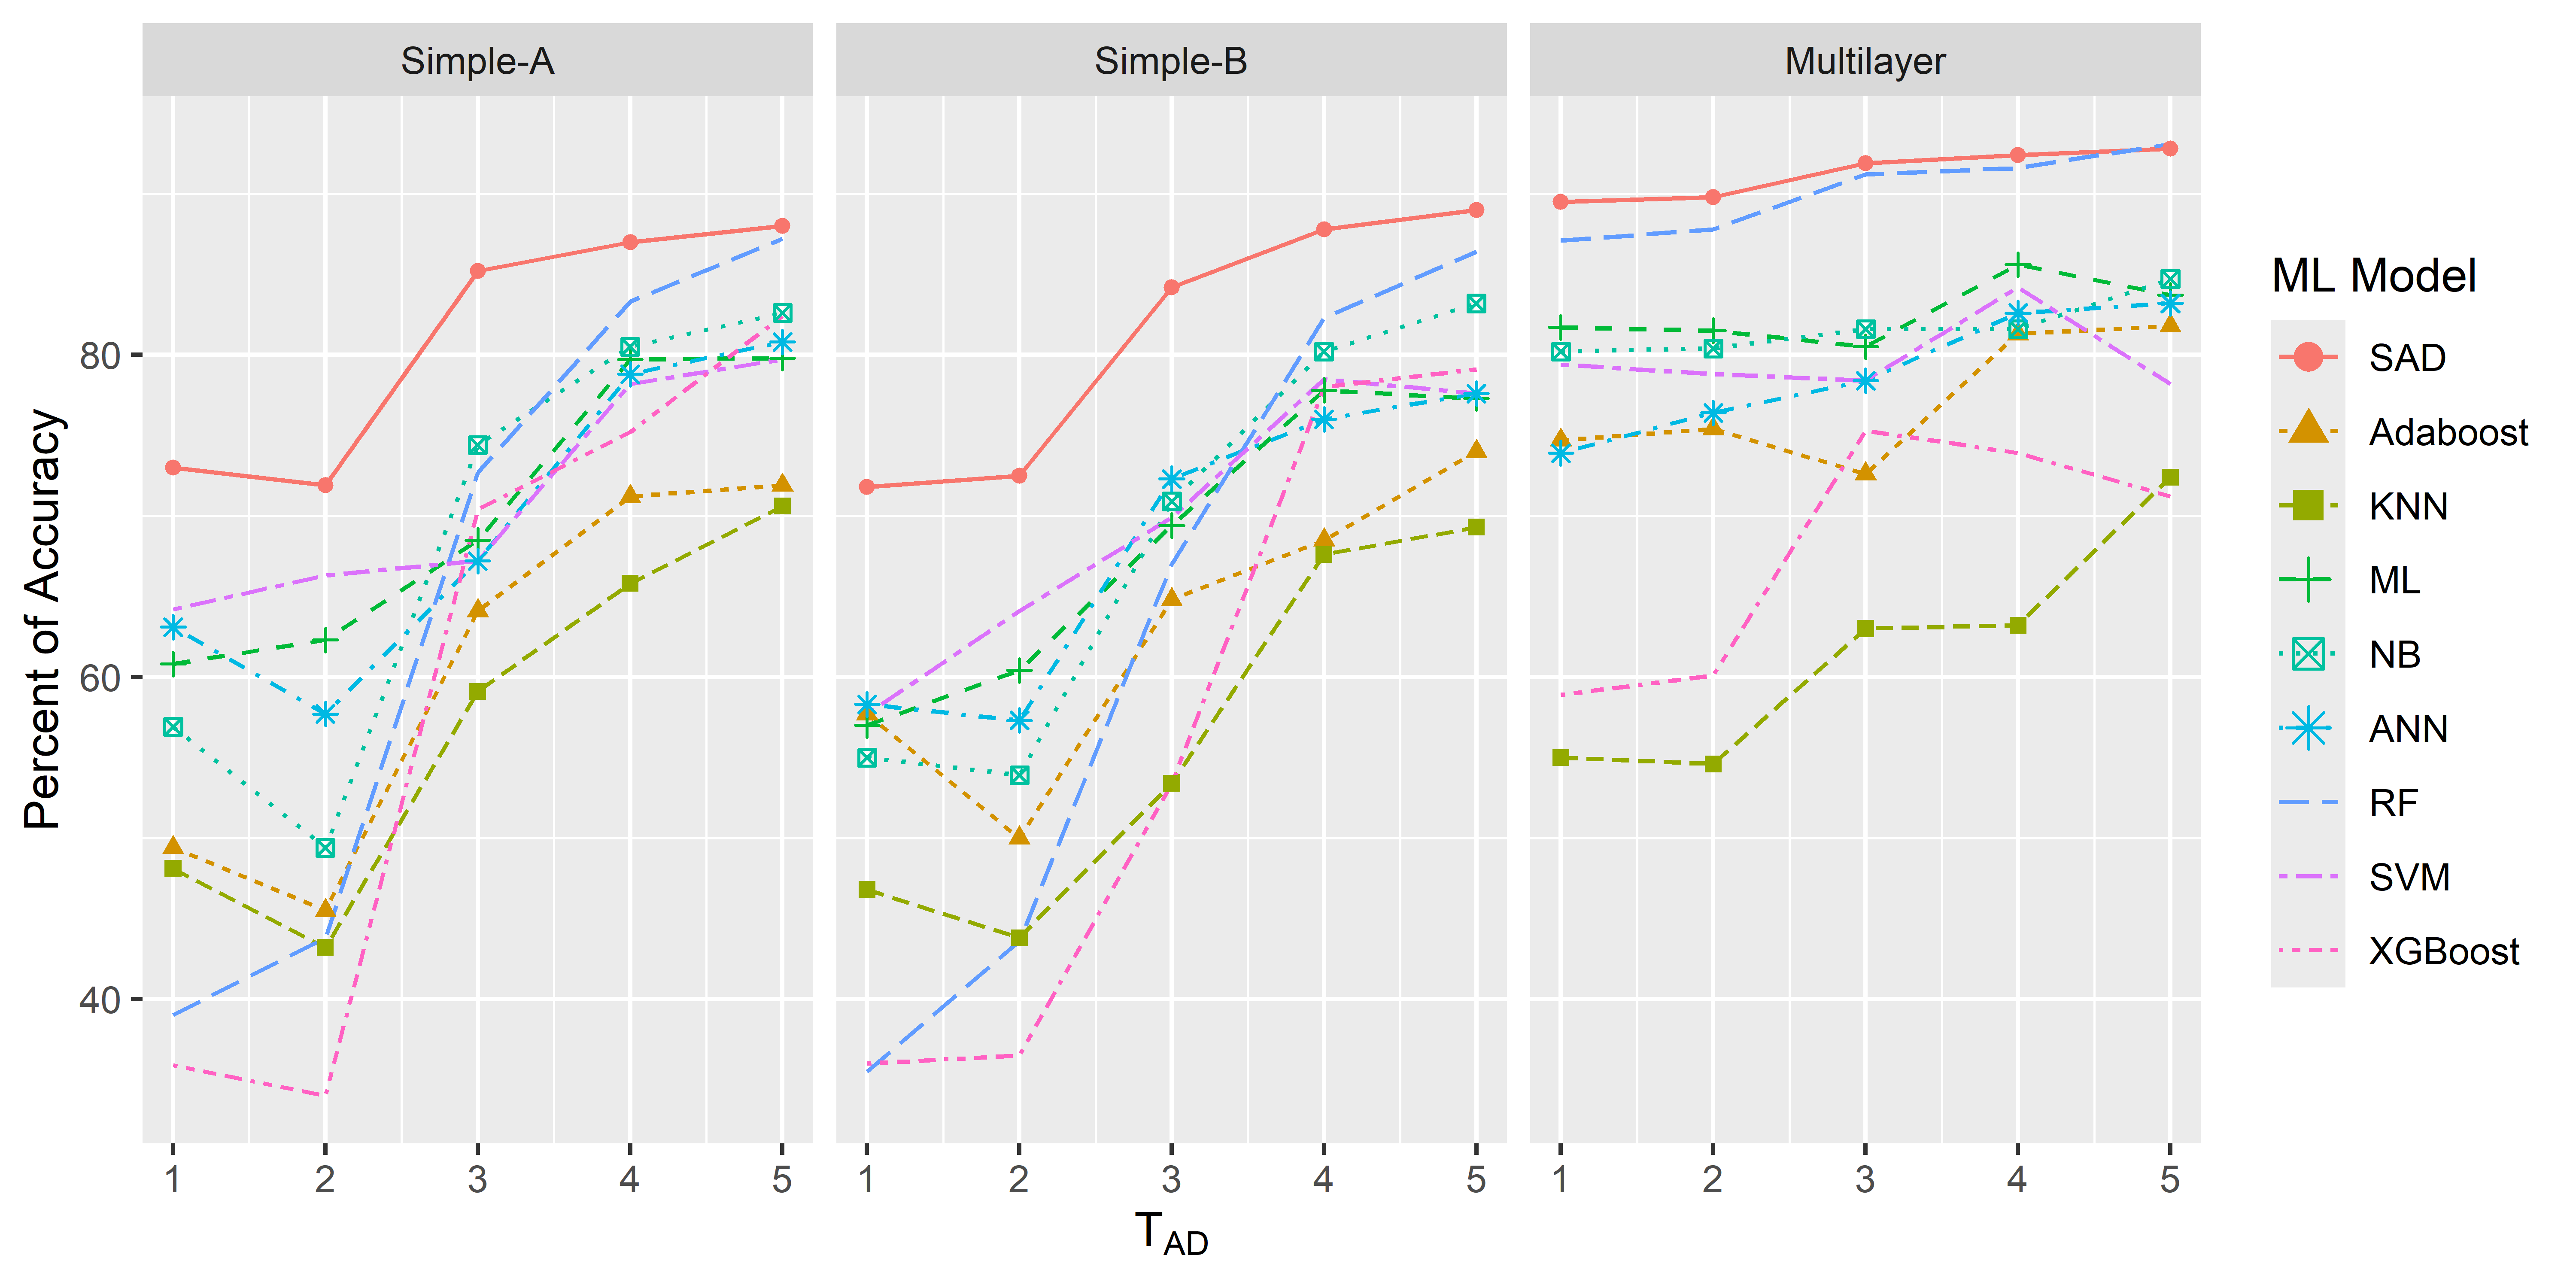
\includegraphics[width=\textwidth]{Pictures/FIG3_1.PNG}

            \caption{The trend of accuracy of algorithms respect to $T_{AD}$ in the second partition  for $T_{ML} = 7 \,, M = 8 $ and different structures.}\label{fig3_1}

        \end{figure}
    \end{center}

In Figure \ref{fig3_1}, with $T_{ML}$ fixed at 7 for the second
partition, the accuracy of various machine learning models within
different structures is depicted. It becomes evident that accuracy
shows a positive correlation with $T_{AD}$ across all machine
learning models. This suggests that increasing the anomaly
detection threshold generally improves the performance of these
models, regardless of the specific structure in which they
operate.

In general, the Multilayered structure of the SAD algorithm consistently outperforms the
other two structures, demonstrating its superior performance.
Furthermore, among the various models analyzed, the SAD model
emerges as the top-performing model across all structures. This
highlights the effectiveness of the SAD model in anomaly detection
tasks within different structural contexts.

    \begin{figure}[H]
        \centering%% For centre alignment of image.
       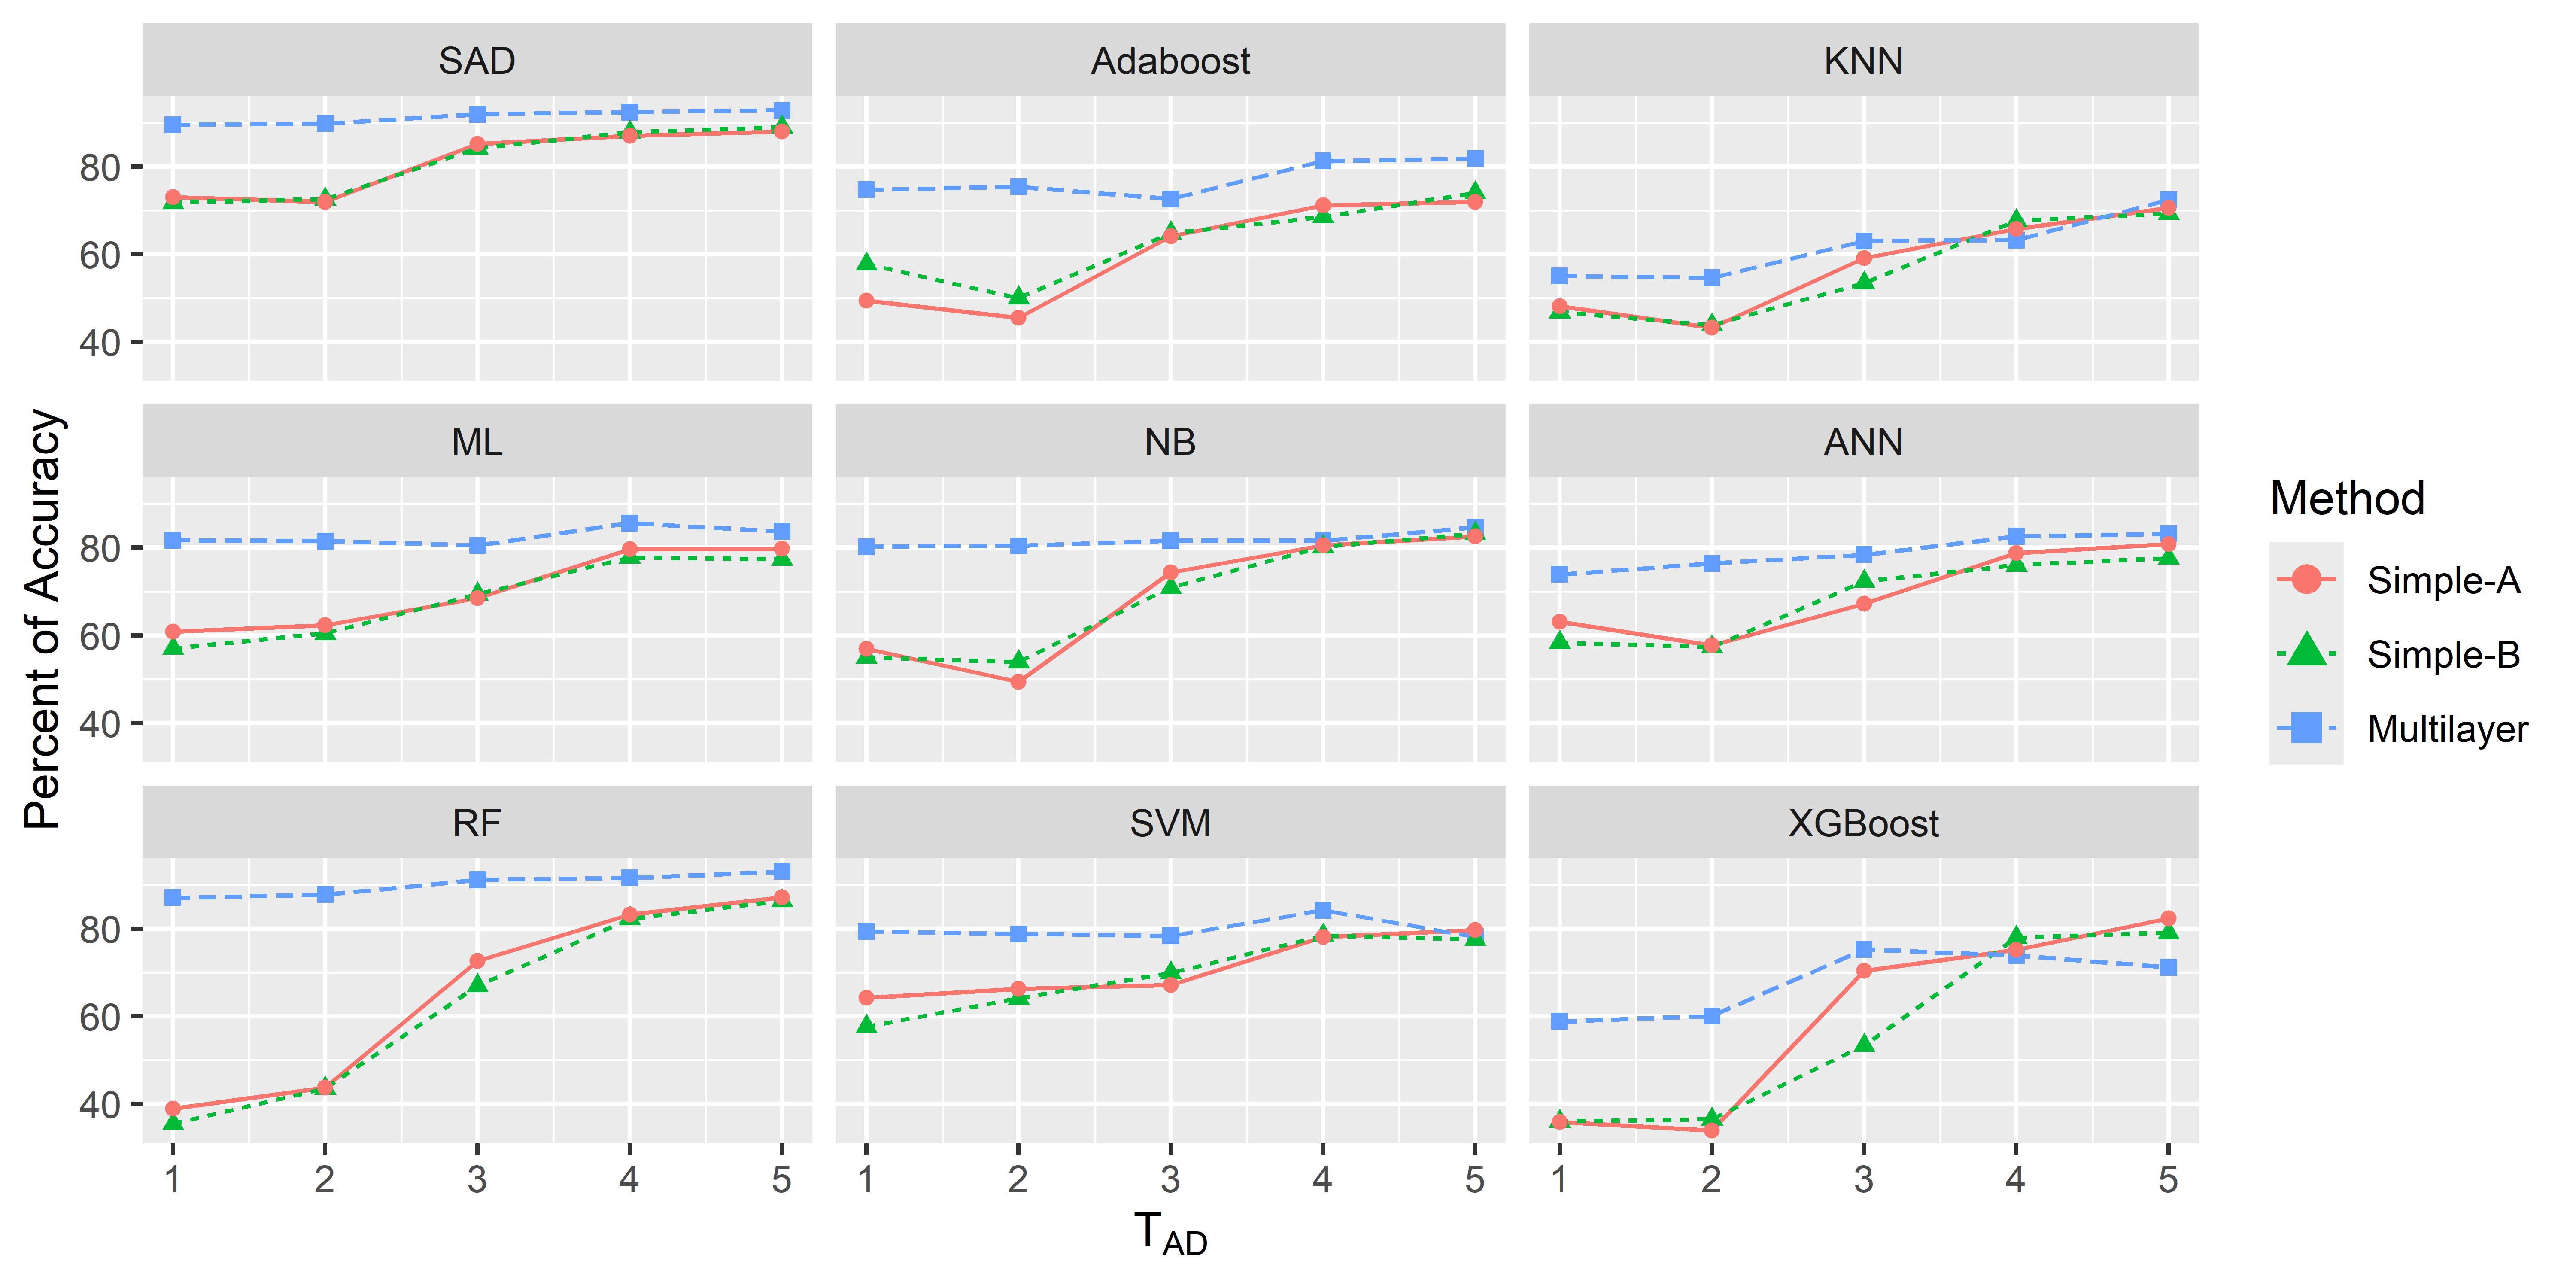
\includegraphics[width=\textwidth]{Pictures/FIG3_2.PNG}
        \caption{Accuracy versus $T_{ML}$ in the fourth partition for $T_{AD}=5$, $M=8$, and different algorithms.}\label{fig3_2}
    \end{figure}

Figure~\ref{fig3_2} compares the architectures as $T_{ML}$ changes in the
fourth partition with $T_{AD}=5$. The multilayer curve is generally above the
two flat alternatives, although the size of the difference depends on the
component learner. This interaction confirms that the placement of EAD, not
only its inclusion, affects the observed threshold response.


    %%FIG4

    \begin{center}
        \begin{figure}[H]%% placement specifier

            \centering
            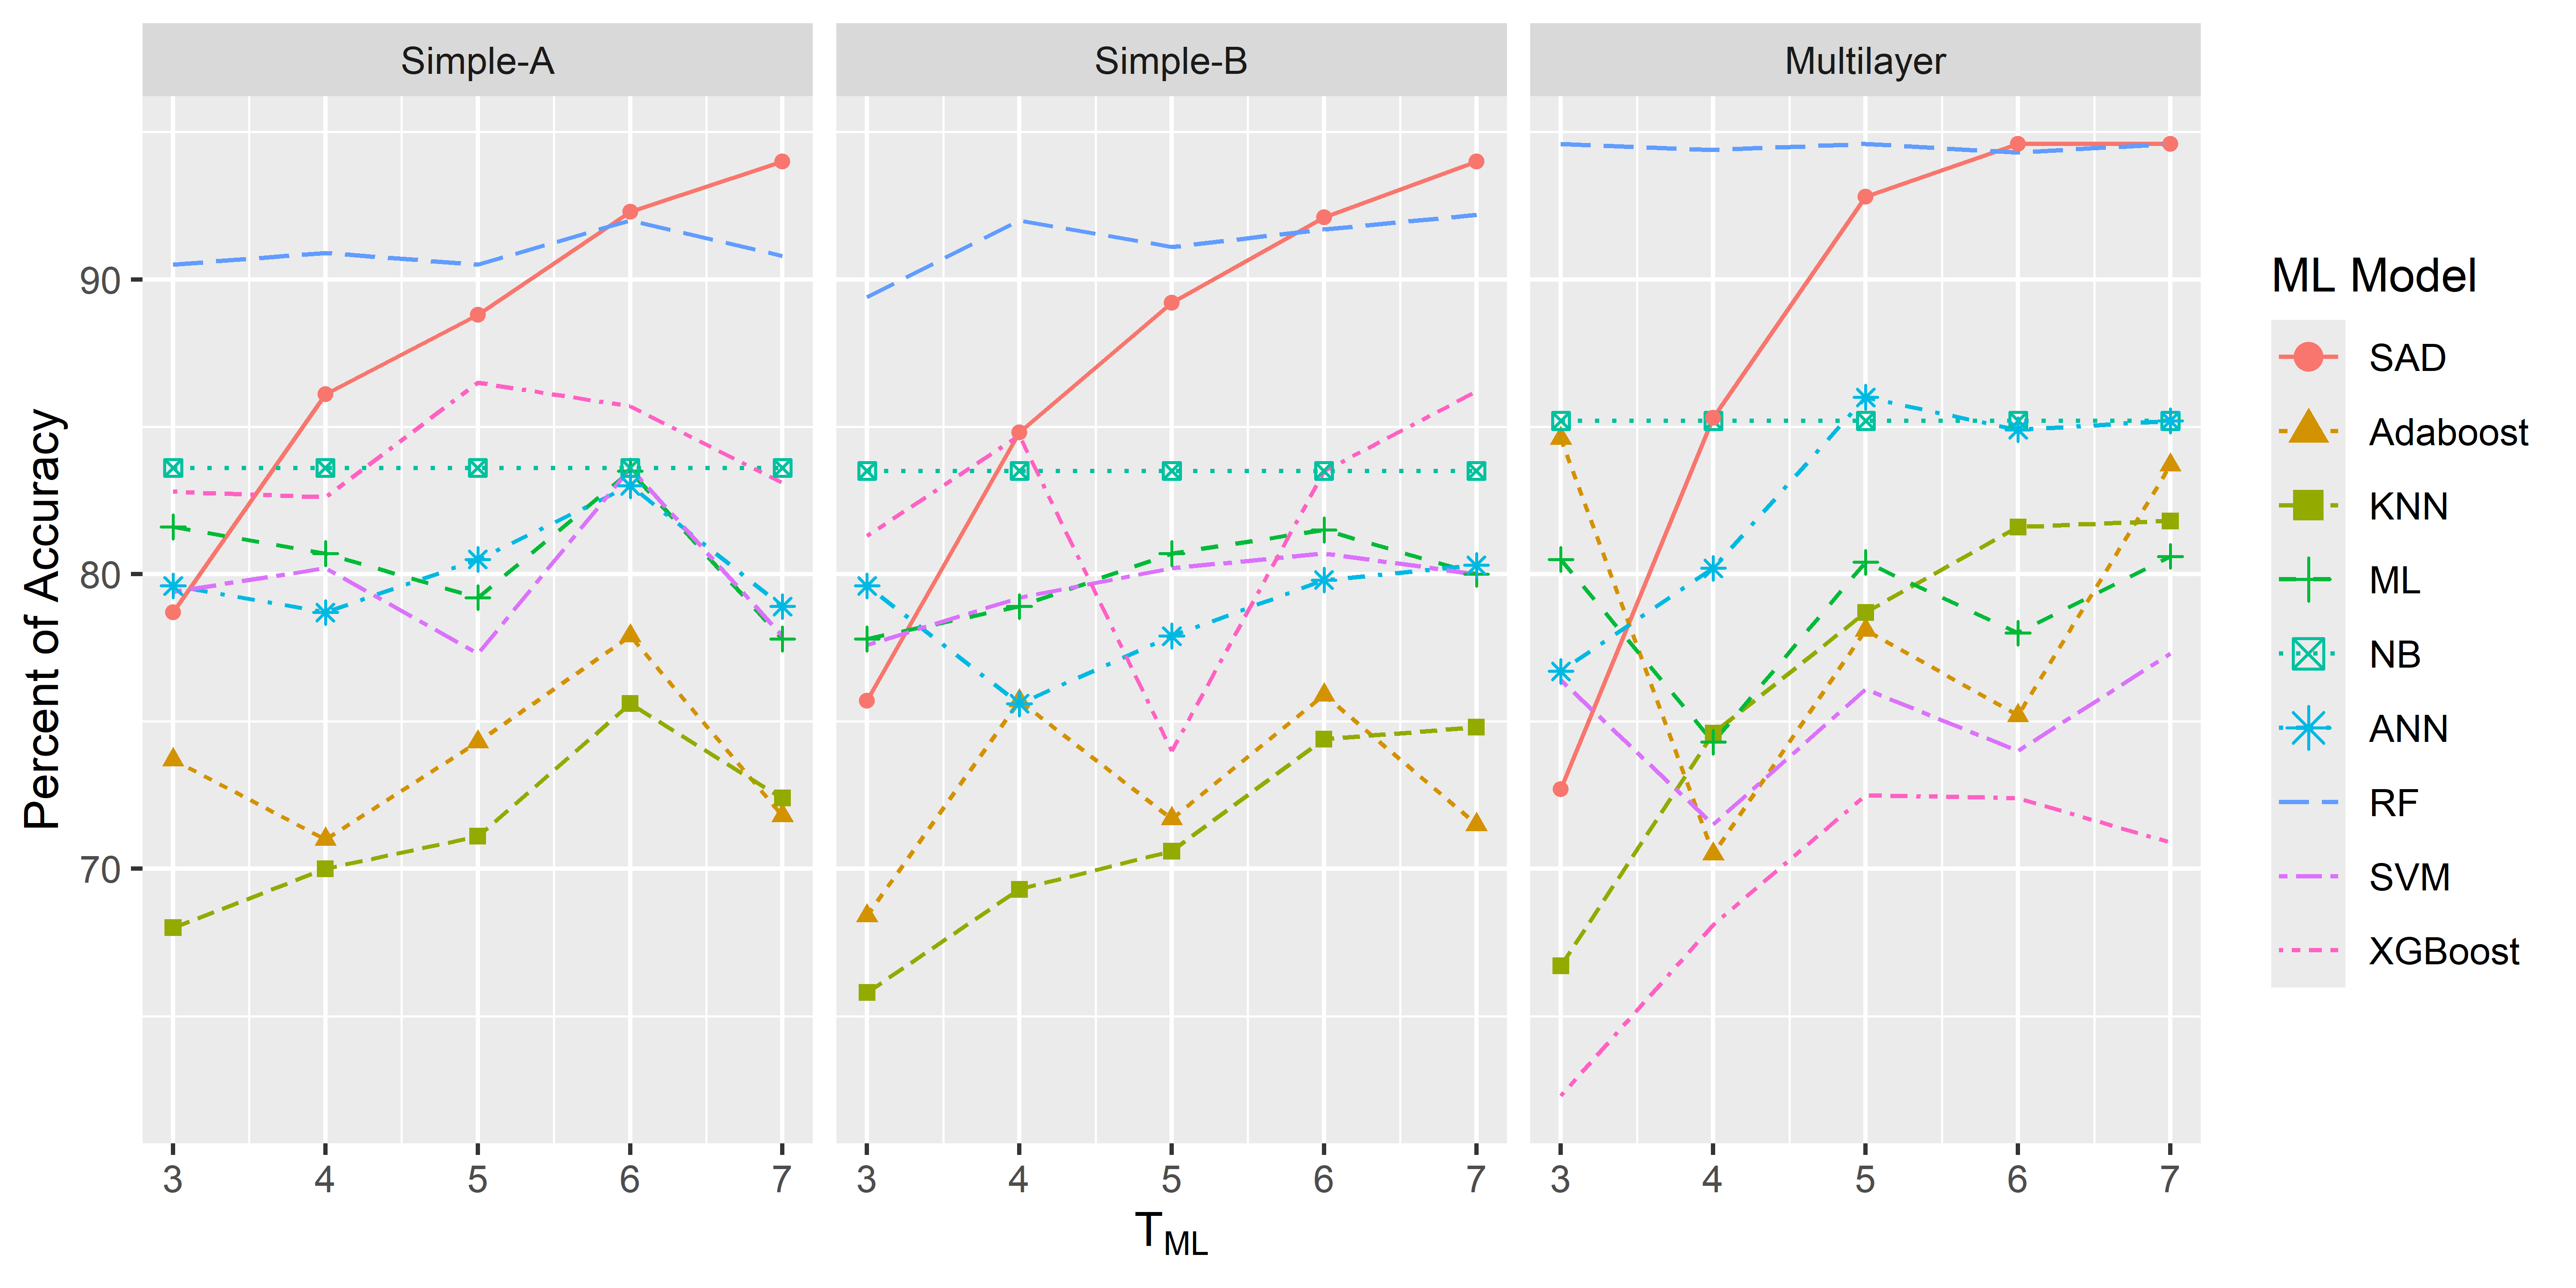
\includegraphics[width=\textwidth]{Pictures/FIG4_1.PNG}

            \caption{Accuracy of the component algorithms versus $T_{ML}$ in the fourth partition for $T_{AD}=5$, $M=8$, and the three architectures.}\label{fig4_1}

        \end{figure}
    \end{center}

In Figure \ref{fig4_1}, with $T_{AD}$ set to 5 for the fourth
partition, we analyze the accuracy of various machine learning
models within different structures. The SAD model displays a
strong correlation between accuracy and $T_{ML}$, while other
machine learning models exhibit a weaker correlation or
fluctuations. Ultimately, the SAD model achieves higher accuracy
across all three structures, underscoring its superior
performance. Additionally, Random Forest and Logistic Regression
models also show some degree of independence from the correlation,
further highlighting the diverse performance characteristics of
these models within different structural contexts.


    \begin{figure}[H]
        \centering%% For centre alignment of image.
       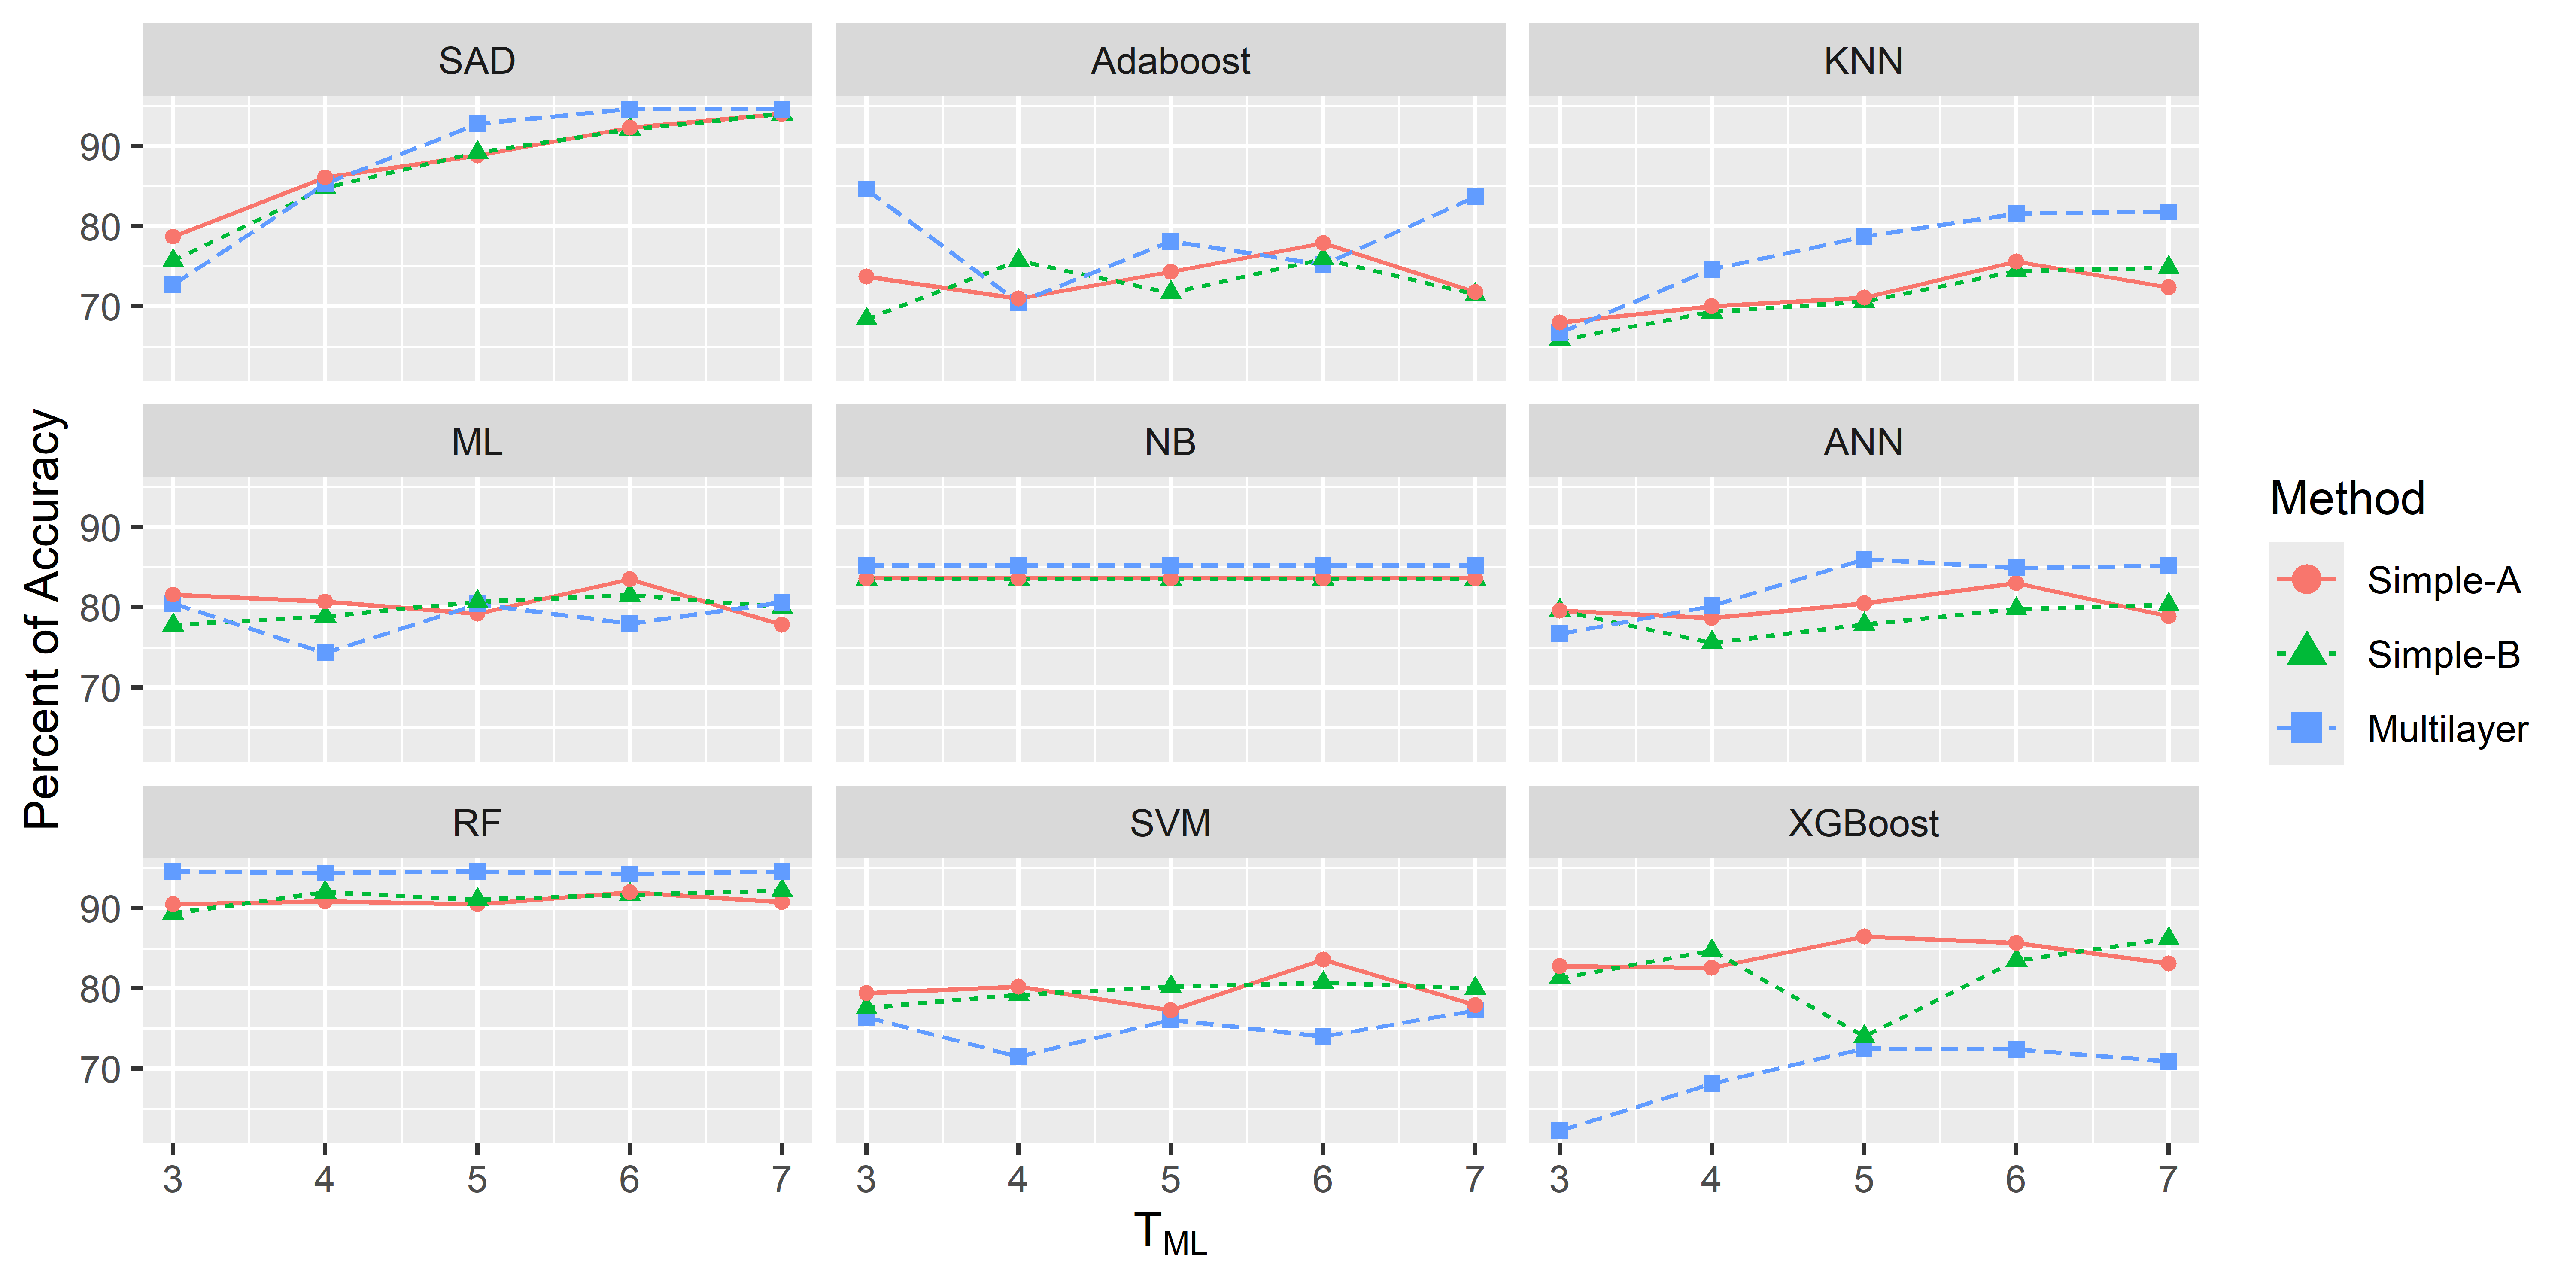
\includegraphics[width=\textwidth]{Pictures/FIG4_2.PNG}
        \caption{Accuracy of the three architectures versus $T_{ML}$ in the fourth partition for $T_{AD}=5$, $M=8$, and different algorithms.}\label{fig4_2}
    \end{figure}

In Figure \ref{fig4_2}, with $T_{AD}$ fixed at 5 for the fourth
partition, the accuracy of various machine learning models within
different structures is depicted. The SAD model shows a positive
correlation between accuracy and $T_{ML}$, whereas other machine
learning models display a weaker correlation. This indicates that
the performance improvement in the SAD model is more directly
connected to increases in $T_{ML}$ compared to other models, which
rely more on $T_{AD}$ adjustments for performance enhancements.

    %%FIG5

    \begin{center}
        \begin{figure}[H]%% placement specifier

            \centering
            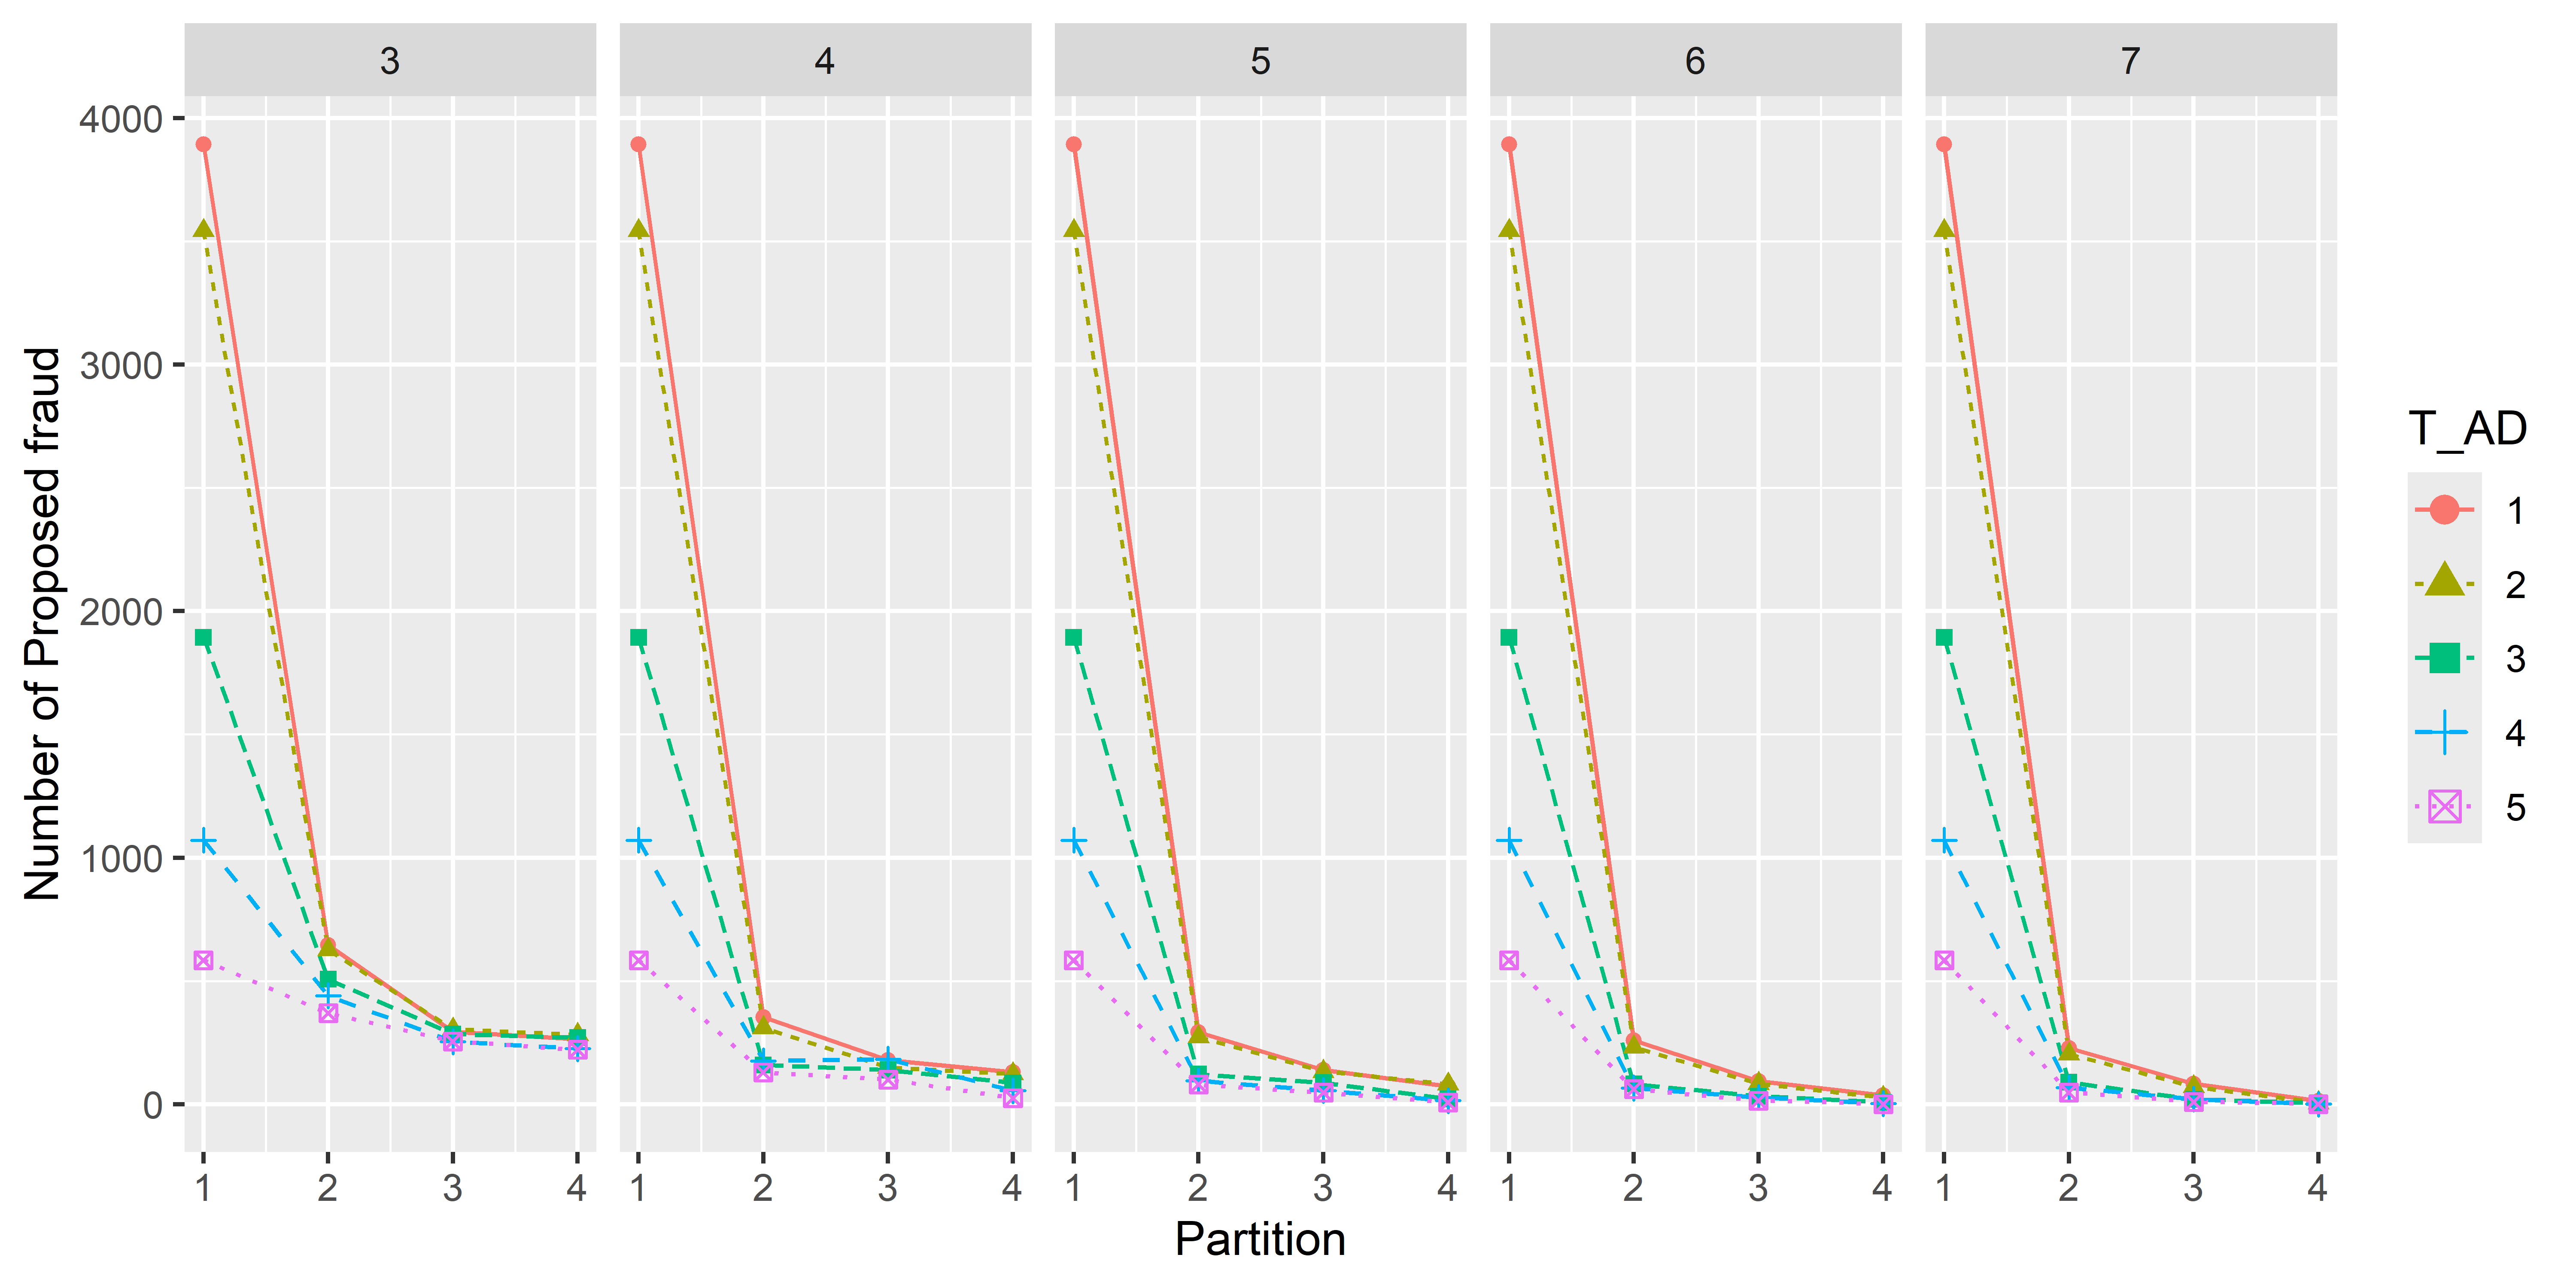
\includegraphics[width=\textwidth]{Pictures/FIG5.PNG}
            \caption{ Number of potential frauds for different values of $T_{AD} \,, T_{ML}$ respect to partition number.  }\label{fig5}
        \end{figure}
    \end{center}

As illustrated in Figure \ref{fig5}, for data sections ranging
from 1 to 4 with varying $T_{ML}$ values, a higher $T_{AD}$
results in fewer data points being sent to the insurance company
for further examination. As the system evolves and $T_{ML}$
progressively increases across sections, the number of data points
requiring expert review significantly decreases, indicating the
improved efficiency and accuracy of the anomaly detection system.

The normal-sampling parameter $PN=10\%$ is used to construct the supervised
training set; it is not itself the proportion of all claims reviewed. The
actual review load is the size of each shortlisted set $F_j$. Figure~\ref{fig5}
shows that stricter voting thresholds reduce that shortlist in this run. This
operational saving must be evaluated jointly with fraud-class recall before a
threshold is selected for deployment.

        \begin{table}[H]
        \centering
        \caption{Elapsed times in each of the partitions with the SAD algorithm for  $T_{ML} = 7 \,, T_{AD} = 5 \,, M = 8$.}
        \label{table1}
        \scriptsize
        \begin{tabular}{llr}
            \hline
            \multicolumn{1}{c}{Partition} & \multicolumn{1}{c}{Structure} & \multicolumn{1}{c}{Time (minutes)} \\
            \hline
            \multicolumn{1}{c}{\multirow{3}{*}{1}} & \multicolumn{1}{c}{Simple-A} & \multicolumn{1}{c}{0.53} \\
            \multicolumn{1}{c}{} & \multicolumn{1}{c}{Simple-B} & \multicolumn{1}{c}{25.18} \\
            \multicolumn{1}{c}{} & \multicolumn{1}{c}{Multilayer} & \multicolumn{1}{c}{1.78} \\
            \hline
            \multicolumn{1}{c}{\multirow{3}{*}{2}} & \multicolumn{1}{c}{Simple-A} & \multicolumn{1}{c}{0.78} \\
            \multicolumn{1}{c}{} & \multicolumn{1}{c}{Simple-B} & \multicolumn{1}{c}{1.03} \\
            \multicolumn{1}{c}{} & \multicolumn{1}{c}{Multilayer} & \multicolumn{1}{c}{0.80} \\
            \hline
            \multicolumn{1}{c}{\multirow{3}{*}{3}} & \multicolumn{1}{c}{Simple-A} & \multicolumn{1}{c}{0.06} \\
            \multicolumn{1}{c}{} & \multicolumn{1}{c}{Simple-B} & \multicolumn{1}{c}{0.07} \\
            \multicolumn{1}{c}{} & \multicolumn{1}{c}{Multilayer} & \multicolumn{1}{c}{0.06} \\
            \hline
            \multicolumn{1}{c}{\multirow{4}{*}{4}} & \multicolumn{1}{c}{Simple-A} & \multicolumn{1}{c}{0.07} \\
            \multicolumn{1}{c}{} & \multicolumn{1}{c}{Simple-B} & \multicolumn{1}{c}{0.09} \\
            \multicolumn{1}{c}{} & \multicolumn{1}{c}{Multilayer} & \multicolumn{1}{c}{0.07} \\
            \hline
            \multicolumn{1}{c}{\multirow{4}{*}{Total}} & \multicolumn{1}{c}{Simple-A} & \multicolumn{1}{c}{1.43} \\
            \multicolumn{1}{c}{} & \multicolumn{1}{c}{Simple-B} & \multicolumn{1}{c}{26.38} \\
            \multicolumn{1}{c}{} & \multicolumn{1}{c}{Multilayer} & \multicolumn{1}{c}{2.71} \\
            \hline
        \end{tabular}
    \end{table}
Table \ref{table1} shows that the first partition requires more
time due to higher data volume and entropy structure
implementation. Simple Structure A is faster due to the absence of
the entropy method, while Simple Structure B takes longer despite
using entropy. The  Multilayered structure of the SAD algorithm significantly reduces time
from 25.18 minutes to 1.78 minutes with an entropy filter layer.
In partitions 2 to 4, no significant differences are observed
between models due to the same $ML\, SET$ implementation. The
upcoming section provides a conclusion and recommendations for
further exploration in this field.

\subsection*{External validity and remaining experimental needs}
\revmark{ADDED --- independent-dataset limitation and validation protocol}
This study uses one static automobile-insurance dataset and one recorded
random partitioning. Consequently, it does not establish transportability to
another insurer, product line, jurisdiction, or time period. Files with
different names but the same Carclaims records would not constitute an
independent dataset, so no such result is presented. A definitive external
validation should freeze the preprocessing rules and thresholds selected on
Carclaims, then evaluate them on a genuinely independent labelled claims
portfolio. Repeated seeds, confidence intervals, fraud-class precision--recall
curves, PR-AUC, review rate, and expected investigation cost should also be
reported. These additions require record-level predictions or a new data-use
agreement and remain necessary before production claims can be made.

\iffalse
\section{CONCLUSION}\label{SC:CONCLUSION}
This study leveraged artificial intelligence and reinforcement
learning to detect insurance fraud. Various algorithms and
structures, including statistical methods and machine learning
models, were presented, leading to the following key findings:
({\bf 1}) Due to time constraints, the entropy method and
information theory are unsuitable for the Simple-B structure, as
all observations in the first data section must be reviewed by the
entire $AD\, SET$; ({\bf 2}) Higher $T_{AD}$ and $T_{ML}$ parameters
improve accuracy across all structures, with more methods employed
in the initial voting process; ({\bf 3}) Increasing $T_{AD}$
reduces the number of observations sent for expert review, while
raising $T_{ML}$ decreases the amount of data sent from the third
section onwards; ({\bf 4}) The SAD method provides the best
accuracy within the dataset, followed by the Random Forest model;
({\bf 5}) Increasing $T_{AD}$ significantly improves accuracy in
the second section, while increasing $T_{ML}$ primarily benefits
the SAD method; ({\bf 6}) The same observations on accuracy also
apply to recall and F1 score.

Recommendations for future research include optimizing utilized
models, exploring different $ML\, SET$s, employing various $AD\, SET $s, and e	xamining diverse logistic regression models. Weighted
voting may also enhance the structures' effectiveness, allowing
more established models and methods to have a greater influence in
the voting process.
\fi

\section{Conclusion}\label{SC:CONCLUSION}
\revmark{REVISED CONCLUSION --- unsupported RL claims replaced}
We introduced SAD as a human-in-the-loop, sequential fraud-screening workflow.
Its sequential contribution is the repeated conversion of verified candidates
into an expanding supervised training set; its multilayer contribution is the
ordered separation of broad anomaly consensus from an entropy-based gate. This
distinction differentiates SAD from a static supervised classifier, a flat
anomaly ensemble, a sequence model, and a reinforcement-learning agent.

On the Carclaims benchmark, the SAD ensemble achieved the strongest reported
within-run metrics, with random forest the strongest individual learner. The
component ablation shows that placing EAD after anomaly consensus can provide a
more favorable accuracy--runtime profile than including it in a flat ensemble:
at the reported operating point, first-partition runtime falls from 25.18 to
1.78 minutes for Simple-B versus Multilayer, while Multilayer attains 0.95
accuracy in partition 4. The threshold grid further demonstrates that
$T_{AD}$ and $T_{ML}$ control both shortlist composition and investigation
load; they should therefore be selected from the business costs of missed fraud
and unnecessary review, not from accuracy alone.

The evidence remains retrospective and single-dataset. Future work should
conduct genuinely independent and prospective validation, repeat experiments
across random seeds, report class-specific confusion matrices and PR-AUC, and
compare review cost at matched fraud recall. Weighted or calibrated voting,
temporal partitions, explicit investigator budgets, and uncertainty-aware
query selection are promising extensions. These steps would test whether the
operational benefits observed here persist under distribution shift and real
expert feedback.

\baselineskip12pt
\bibliographystyle{apalike}    % Choose your desired style
\bibliography{refs}

\end{document}
